\chapter{Related Work}
homotopy switching model \citep{evrard2009homotopy}, admittance master slave example \citep{tagliabue2017collaborative}.

\begin{figure}[h]
   \centering
   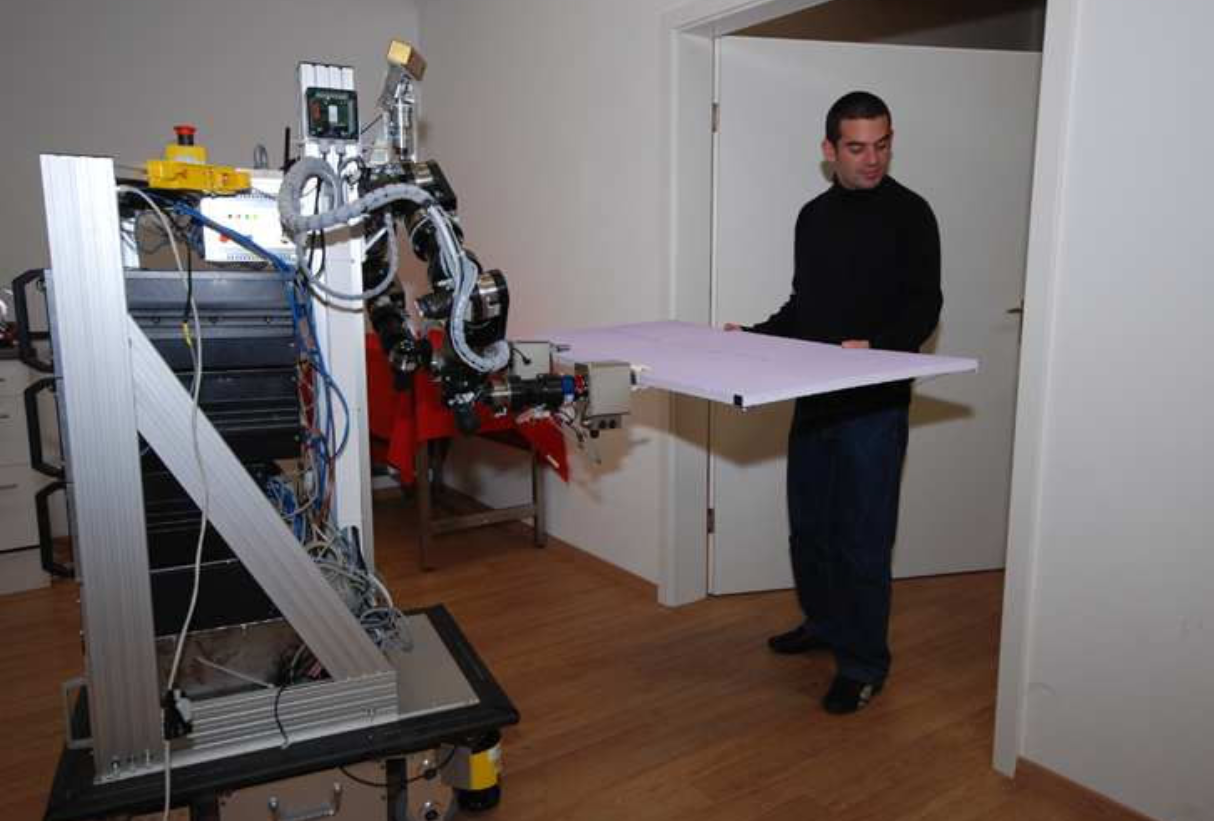
\includegraphics[width=0.75\textwidth]{images/lawitzky2010.png}
   \caption{Load sharing example \citep{lawitzky2010load}.}
   \label{pics:lawitzky2010}
\end{figure}

\chapter{The Thing Mobile Manipulator}
We conduct our research on a mobile manipulator, lovingly called the \emph{Thing} and depicted in Figure \ref{pics:thing}. It is composed of three main components and various sensing technologies, on which we elaborate in detail in this chapter. The three components, from bottom to top, are a Ridgeback omnidirectional robot platform \citep{ridgeback}, a UR10 robotic arm \citep{ur10} and a Robotiq three finger gripper \citep{robotiqGripper}.

\begin{figure}[h]
   \centering
   \includegraphics[width=0.75\textwidth]{images/thing.jpg}
   \caption{The Thing mobile manipulator, which consists of a Ridgeback omnidirectional platform, a UR10 and a Robotic gripper.}
   \label{pics:thing}
\end{figure}

These hardware packages are essentially independent and are interfaced in a central computing unit, located in the ridgeback. The interface is achieved using a Robot Operating System (ROS) server, which also acts as the user interface. It allows for information sharing between the system and access for the user on high and low system levels.

The rich and easily expandable sensing equipments include wheel odometry, an Inertial Measurement Unit (IMU) and a Hokuyo laser range finder (LIDAR) \citep{hokuyo} in the Ridgeback and a FT 300 force torque sensor \citep{robotiqFT300} in between the gripper and the UR10.

The omnidirectional capability together with the modularity of the system and the vast amount of sensor arrays make the Thing mobile manipulator a popular and widely used system for autonomous robotics research.

The whole manipulator is an out of the box system assembled by Clearpath, which collaborates with Universal Robots and Robotiq and mounts the parts on the platform in house.

\section{Clearpath Ridgeback}
	\label{sec:ridgeback}
The Ridgeback, depicted in Figure \ref{pics:ridgeback} is an omnidirectional robot platform designed by Clearpath for indoor movement and payload carrying tasks, such as autonomous warehousing for example. It is a fully integrated system with sensors, actuation and control and features a native ROS interface. The wheel odometry provides accurate localization and can be fused with the front facing LIDAR and IMU for obstacle avoidance and SLAM implementations, which are implemented for example in the ROS navigation stack. Optionally, a second rear facing LIDAR can be mounted for full \unit[360]{\textdegree} coverage. Specifications are summarized in Table \ref{tab:ridgeback}.

\begin{figure}[h]
   \centering
   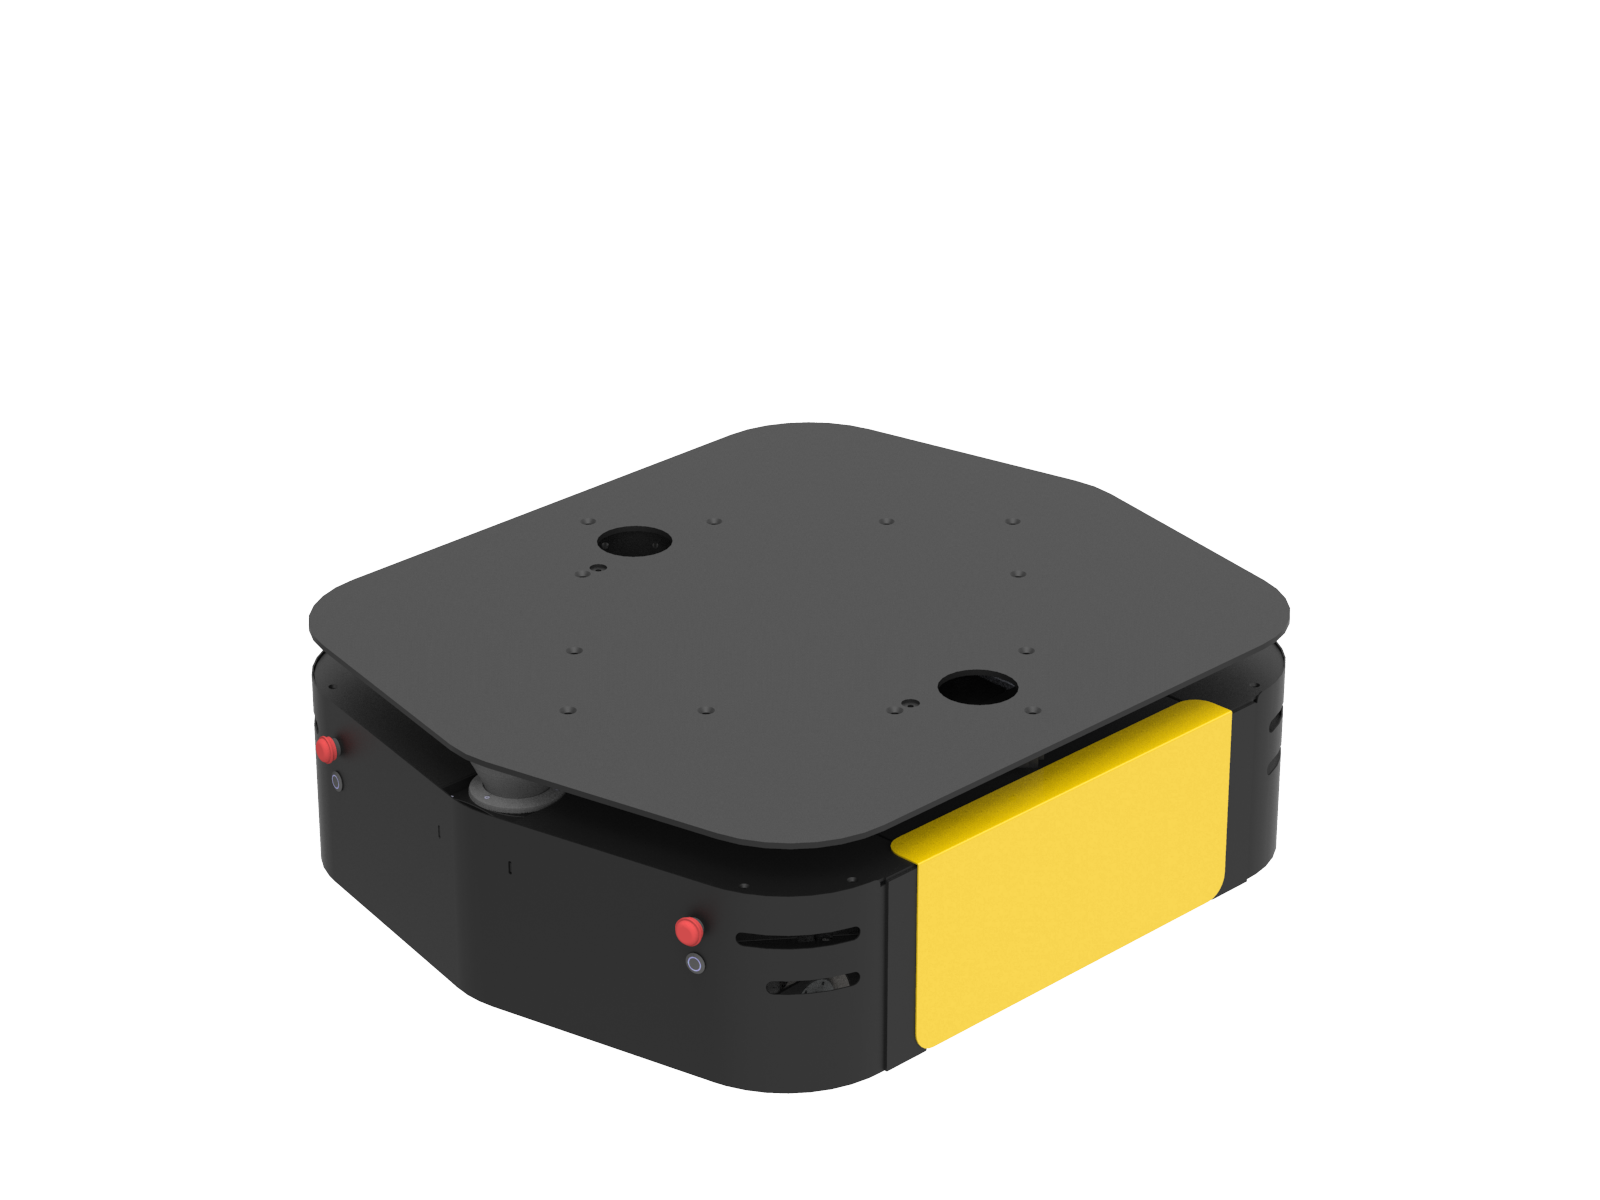
\includegraphics[width=0.75\textwidth]{images/ridgeback.png}
   \caption{Clearpath Ridgeback}
   \label{pics:ridgeback}
\end{figure}

\begin{table}[h]
\begin{center}
 \caption{Clearpath Ridgeback Specifications}\vspace{1ex}
 \label{tab:ridgeback}
 \begin{tabular}{ll}
 \hline
 Length & \unit[960]{mm}\\
 Width & \unit[793]{mm}\\
 Height & \unit[296]{mm}\\
 Weight & \unit[135]{kg}\\
 Maximum payload & \unit[100]{kg}\\
 Maximum velocity & \unitfrac[1.1]{m}{s}\\
 Average power consumption & \unit[800]{W}\\
 Drivers and APIs & ROS \\
 Sensors & Wheel odometry\\
 & Inertial measurement unit (IMU) \\
 & Laser range finder LIDAR \\
 \hline
 \end{tabular}
\end{center}
\end{table}

The broad range of sensors, it's flexibility and low drift in odometry makes the Ridgeback a suitable and popular platform for research in controlled indoor environments.

Because the Ridgeback is omnidirectional, it has three degrees of freedom (DOF) and can move instantaneously along the two linear horizontal axes $x$ and $y$, as well as rotate around the vertical axis $z$, which is expressed by the yaw angle $\theta$. 

Additionally, the Ridgeback houses the on-board computer that runs the low-level drivers of all the elements of the manipulator. On top thereof, there is a high-level driver that ensures accord and offers a ROS interface for the user to connect to.

\section{Universal Robot 10}
The UR10 is a collaborative industrial robot arm by Universal Robots. It has six rotary joints, hence six DOF and can support payloads up to \unit[10]{kg}. Together with it's little brother the UR5, it is widely regarded as the standard manipulator within robotics research. Hence, extensive platform and software integration resources are available and ROS is supported out of the box.

As we see in Table \ref{tab:ur10}, the repeatability of \unit[0.1]{mm} allows for repeatedly achieving a pose with high accuracy, which is important for industrial and research applications alike.

\begin{figure}[h]
   \centering
   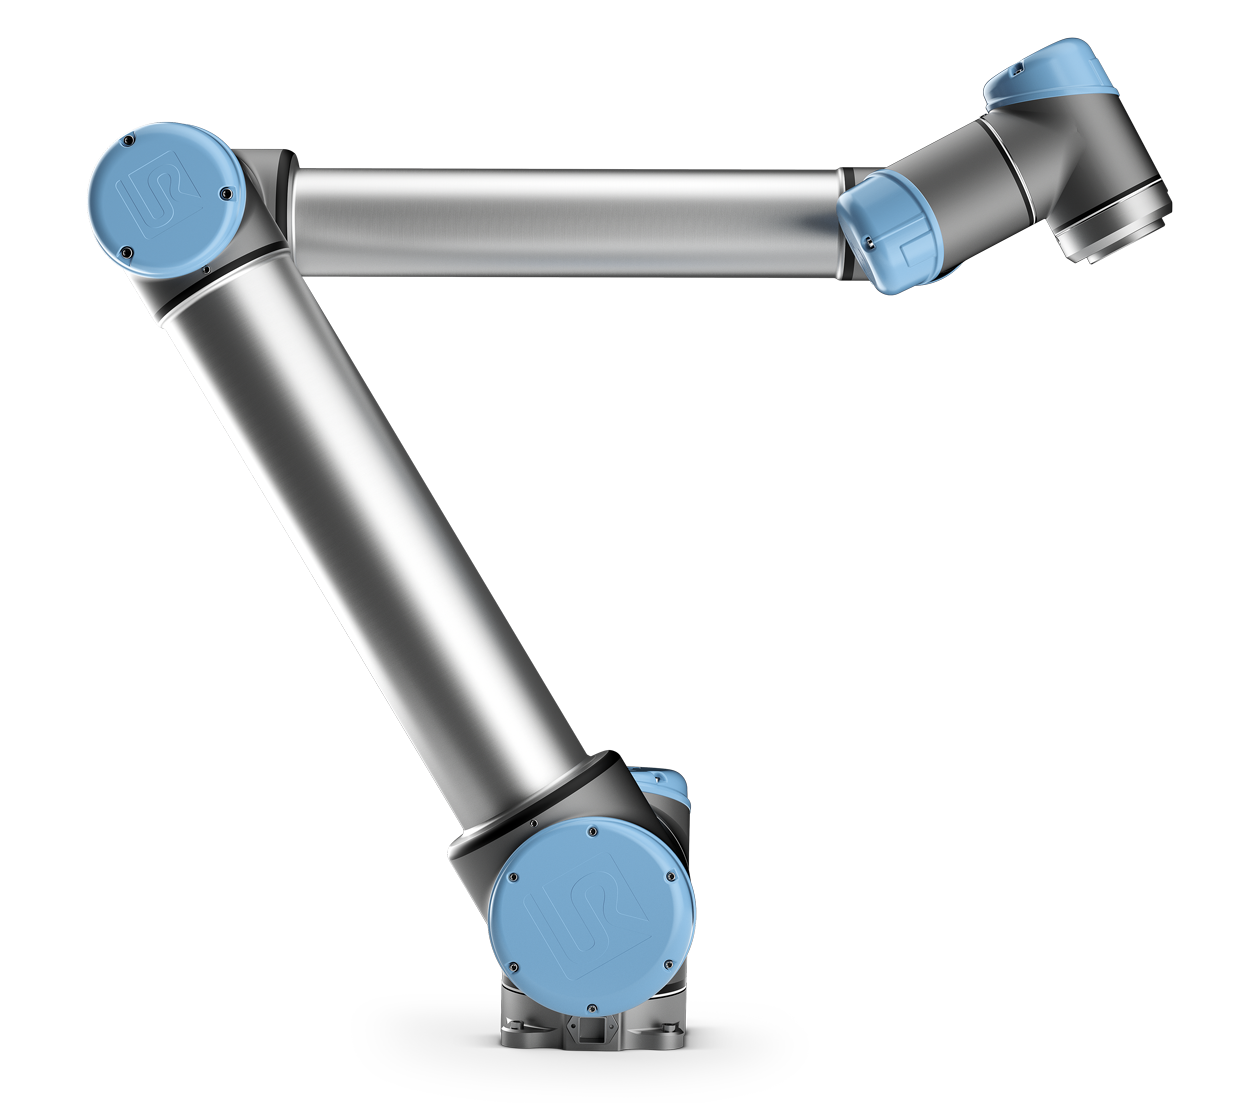
\includegraphics[width=0.75\textwidth]{images/ur10.png}
   \caption{Universal Robot 10}
   \label{pics:ur10}
\end{figure}

\begin{table}[h]
\begin{center}
 \caption{Universal Robot 10 Specifications}\vspace{1ex}
 \label{tab:ur10}
 \begin{tabular}{ll}
 \hline
 Reach & \unit[1300]{mm} \\
 Weight & \unit[1.5]{kg}\\
 Repeatability & \unit[0.1]{mm} \\
 Maximum payload & \unit[10]{kg}\\
 Maximum tool velocity & \unitfrac[1]{m}{s}\\
 Degrees of freedom & 6 rotating joints \\
 Average power consumption & \unit[350]{W}\\
 \hline
 \end{tabular}
\end{center}
\end{table}

\section{Robotiq Three Finger Gripper}
The Robotiq three finger adaptive gripper, depicted in Figure \ref{pics:robotiq_gripper}, is the end-effector mounted on the UR10 on the Thing. As specified in Table \ref{tab:robotiq_gripper}, it has four different grip types and allows for force, position and speed control for each finger individually. This makes it suitable for manufacturing, assembly, pick and place and other research applications.

\begin{figure}[h]
   \centering
   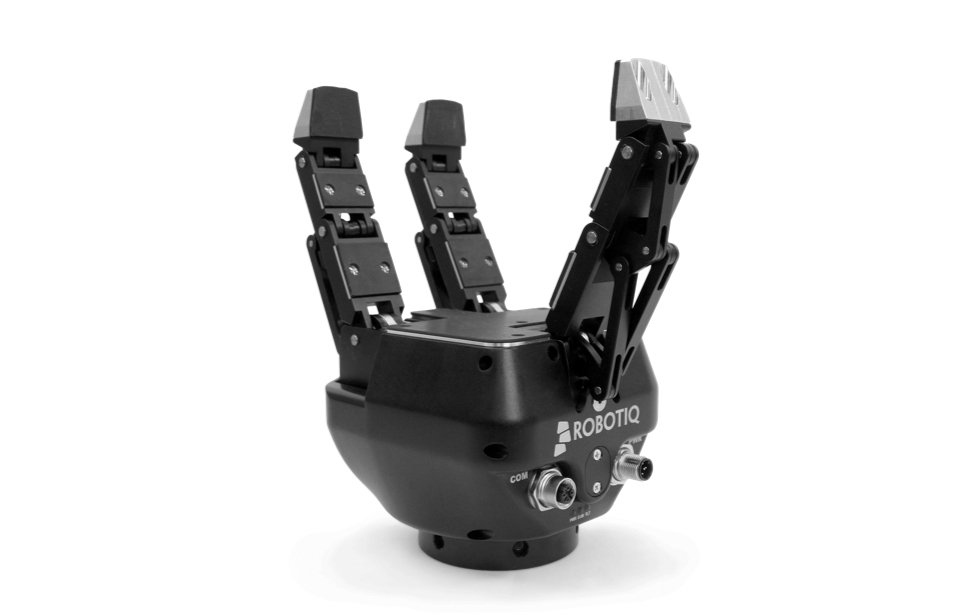
\includegraphics[width=0.75\textwidth]{images/robotiq_gripper.jpg}
   \caption{Robotiq three finger adaptive robot gripper}
   \label{pics:robotiq_gripper}
\end{figure}

\begin{table}[h]
\begin{center}
 \caption{Robotiq 3-Finger Adaptive Robot Gripper Specifications}\vspace{1ex}
 \label{tab:robotiq_gripper}
 \begin{tabular}{ll}
 \hline
 Weight & \unit[2.3]{kg}\\
 Repeatability & \unit[0.1]{mm} \\
 Maximum payload (encompassing grip) & \unit[10]{kg}\\
 Gripper opening & \unit[0 to 155]{mm} \\
 Object diameter for encompassing & \unit[20 to 155]{mm}\\
 Grip force & \unit[30 to 70]{N} \\
 Grip types & Pinch mode \\
 & Wide mode \\
 & Scissor mode \\
 & Basic mode \\
 Minimum power consumption & \unit[4.1]{W} \\
 Peak power (at maximum gripping force) & \unit[36]{W}\\
 \hline
 \end{tabular}
\end{center}
\end{table}

\section{Robotiq FT 300 Force-Torque Sensor}
	\label{sec:ft300}
The FT 300 is a force torque sensor by Robotiq, embedded in a cylindrical and stiff casing. As Figure \ref{pics:robotiq_ft} shows, the sensor is compatible with any Robotiq gripper and Universal Robots arm and acts as an intermediate module between the gripper and the end-effector of the robotic arm. Hence, any force or torque which is transferred from gripper to the arm or vice versa can be measured. The sensor measures forces along and torques around the three axis $x$, $y$ and $z$ of the module, makint it a six dimensional sensor, outputting data at \unit[100]{Hz}. In Table \ref{tab:robotiq_ft}, the measuring ranges and signal noises are listed.

The FT-300 allows for any tasks that make use of force feedback or force control, such as assembly, finishing, insertion, pick and place or teach and repeat applications.


\begin{figure}
   \centering
   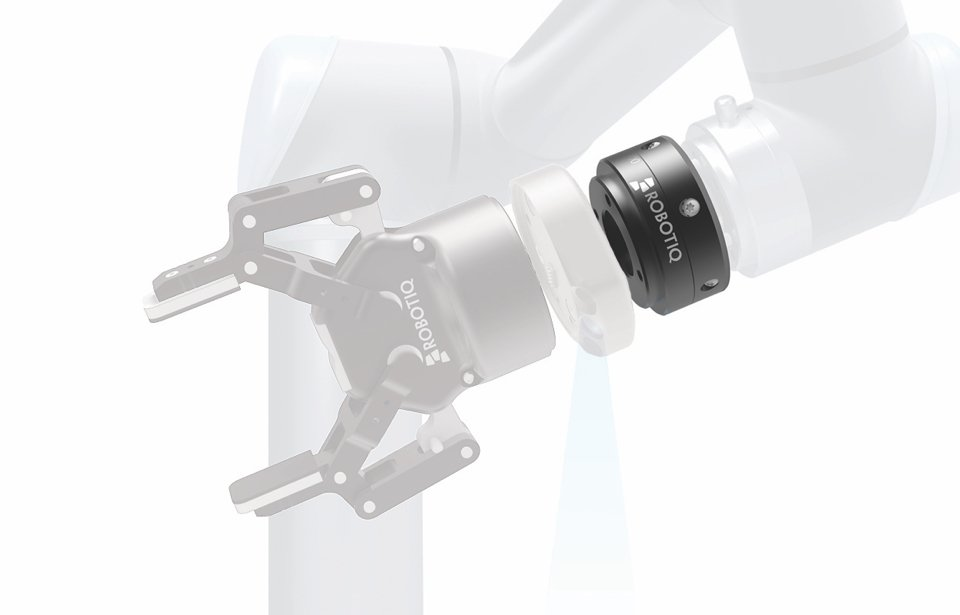
\includegraphics[width=0.75\textwidth]{images/robotiq_ft.jpg}
   \caption{Robotiq FT 300 Force Torque Sensor}
   \label{pics:robotiq_ft}
\end{figure}

\begin{savenotes}
\begin{table}[h]
\begin{center}
 \caption{Robotiq FT 300 Force Torque Sensor Specifications}\vspace{1ex}
 \label{tab:robotiq_ft}
 \begin{tabular}{ll}
 \hline
 \textbf{Measuring range} & \\
 Force $F_x, F_y, F_z$ & \unit[$\pm 300$]{N} \\
 Moment $M_x, M_y, M_z$ & \unit[$\pm 30$]{Nm} \\ \hline
 \textbf{Signal noise}\footnote{Signal noise is the standard deviation of the signal measured over a period of one second.} &\\
 Force $F_x, F_y, F_z$ & \unit[0.1]{N} / \unit[1]{N} \\
 Moment $M_x, M_y$ & \unit[0.05]{Nm} / \unit[0.02]{Nm} \\
 Moment $M_z$ & \unit[0.03]{Nm} / \unit[0.01]{Nm} \\ \hline
 Data output rate & \unit[100]{Hz} \\
 Weight & \unit[300]{g}\\
 Outside diameter & \unit[75]{mm} \\
 Thickness & \unit[37.5]{mm} \\
 \hline
 \end{tabular}
\end{center}
\end{table}
\end{savenotes}

\section{Hokuyo Laser Range Finder}
Figure \ref{pics:hokuyo} depicts the Hokuyo UST-10LX scanning laser range finder. It scans a single horizontal plane by spinning around its vertical axis at \unit[2400]{rpm}, which results in a scanning frequency of \unit[40]{Hz}, also shown in Table \ref{tab:hokuyo}. Compared to any LIDAR system that stacks multiple lasers on top of each other, the Hokuyo UST-10LX is in a disadvantage, because it only outputs two-dimensional range measurements and supplies no information along its vertical axis. However, it outperforms many alternatives in terms of size, weight, power consumption, accuracy and measurement frequency, which makes it highly suitable for a mobile platform.


\begin{figure}[h]
   \centering
   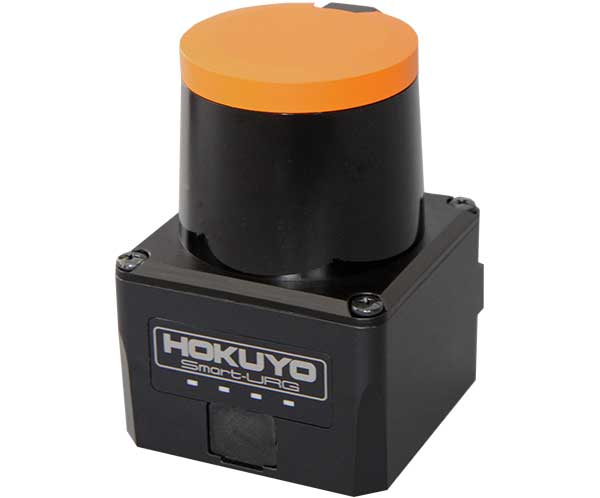
\includegraphics[width=0.75\textwidth]{images/hokuyo.jpg}
   \caption{Hokuyo UST-10LX laser range finder}
   \label{pics:hokuyo}
\end{figure}

\begin{table}[h]
\begin{center}
 \caption{Hokuyo UST-10LX Laser Range Finder Specifications}\vspace{1ex}
 \label{tab:hokuyo}
 \begin{tabular}{ll}
 \hline
 Scan angle & \unit[250]{$\degree$} \\
 Measurement steps & 1081 \\
 Angular resolution & \unit[0.25]{$\degree$} \\
 Detection range & \unit[0.06 to 10]{m} \\
 Scan frequency & \unit[40]{Hz} \\
 Average power consumption & \unit[3]{W} \\
 Weight & \unit[130]{g} \\
 Length & \unit[50]{mm} \\
 Width & \unit[50]{mm} \\
 Height &  \unit[70]{mm} \\
 \hline
 \end{tabular}
\end{center}
\end{table}

\chapter{Admittance Control}
	\label{sec:adm_ctrl}
The term admittance is closely coupled to impedance \citep{hogan1985impedance}.

The interaction between force input and motion output is modeled as a second order spring mass damper system according to Newton's second law of motion, which states that the change in momentum is equal to the sum of all forces acting on our rigid body

\begin{equation}
M \cdot \ddot{X} = \sum F
	\label{eq:virt_work}
\end{equation}
The forces in the case of a mass spring damper system are
\begin{equation}
\sum F = F_D + F_K + F_{ext}
	\label{eq:f_sum}
\end{equation}
which consists of a spring term
\begin{equation}
F_K = K \cdot X
\end{equation}
with spring constant $K$, a damping term
\begin{equation}
F_D = D \cdot \dot{X}
\end{equation}
with damping constant $D$ and a term $F_ext$ for external forces acting on the body. Replacing $\sum F$ in Equation \ref{eq:virt_work} with Equation \ref{eq:f_sum} and dividing by $M$ yields the equation for a second order mass spring damper system:
\begin{equation}
\ddot{X} = M^{-1}(F_{ext} -D \cdot \dot{X} -K \cdot X)
	\label{eq:mass_spring_damper_sys}
\end{equation}




\chapter{Obstacle Avoidance}
Ever since robots faced the task of autonomous navigation, obstacle avoidance has been a crucial element of it. There are numerous approaches to tackle the problem, varying in degrees of foresight and influence on the path planner.

The problem can be seperated into two categories, path planning around obstacles on a global scale and on a local scale. The first category bundles algorithms that take a goal position and a current position of a robot and calculate the optimal path (usually the shortest path) in between, given some objective function and a map. Since the distance to the goal is normally greater than the range of any obstacle detection sensor, these algorithms need a full map of the environment. Widely used examples are A*, Djikstra, Bit* and RRT.

In contrast, path planning on a local scale takes obstacle detection sensor information as an input and outputs commands to a drive unit, that meet the given objective, which is usually to avoid collisions and stay clear of an obstacle by a minimum distance. 

A typical path planning infastructure on a robot consists of both a global and a local planner, where the global planner outputs a path to follow to the local planner, which in terms fuses that path with online obstacle detection sensor information to ensure it is indeed collision free and deviates from it if necessary.

To find the path planning algorithm that best meets our needs, we must first examine what are the given inputs and the desired outputs of our system. As we already elaborated in \cref{sec:introduction}, we are working in a master-slave scenario, which means that the robot is trying to achieve the goal of its human counterpart and not its own. This manifests in the planner in such a way, that the input is the force and torque applied by the human and the robot has no global goal pose. Hence, we are inherently bound to iteratively updated goals within close proximity and there is no possibility nor need to apply global path planning techniqes and we focus only on local planners in the remainder of this chapter.

\section{Local Planners}
In this chapter, we discuss a selection of common local planning methods and their feasibility for the task at hand.

%\subsection{Velocity Obstacles}
%Velocity Obstacles (VO) \citep{fiorini1998motion}
%\begin{equation}
%p_{RO} + v_R t < r_R +r_O
%	\label{eq:vo_condition}
%\end{equation}
%\begin{equation}
%VO_{RO} = D TODO fill in
%\end{equation}

\subsection{Dynamic Window Approach}
The Dynamic Window Approach (DWA) \citep{fox1997dynamic} is a well-known algorithm that produces command velocities for a planar robot given vehicle dynamics and obstacle measurements. The basic assumption is that the robot moves instantaneously on circular arcs with a translational velocity $v$ and a rotational velocity $\omega$. Thus, the complexity is greatly simplified and calculations are be performed in the 2D velocity space $(v,\omega)$. Within this space, we compute three sets of velocity pairs,  subsequently called \emph{windows} for every iteration of the algorithm. Figure \ref{pics:dwa} provides a visual example of the functionality of the algorithm.

\begin{description}
\item[Static window] The static window $V_s$ expresses the constraint velocities of the vehicle, i.e., absolute maximum and minimum velocity. As the name suggests, these parameters are usually static and do not need to be recalculated every step.

\item[Obstacle window] The obstacle window $V_o$ are the measurements of any obstacles, e.g. taken by a range laser sensor and transformed from Cartesian to $v,\omega$ space.

\item[Dynamic window]The dynamic window $V_d$ are the vehicle dynamics, i.e., velocities that are physically feasible for the robot to reach within one time step. It's size is defined by the maximal acceleration and the current velocity of the robot.
\end{description}

\begin{figure}[h]
   \centering
   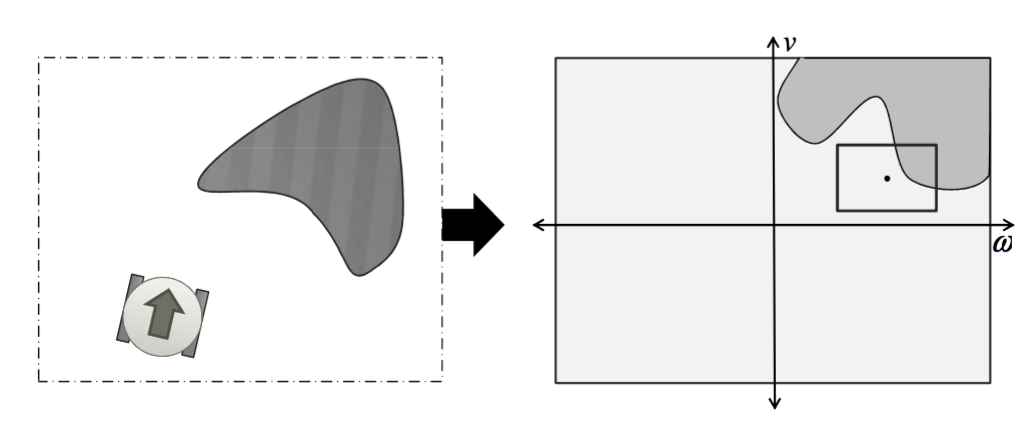
\includegraphics[width=0.75\textwidth]{images/dwa.png}
   \caption{DWA working principle \citep{siegwart2004autonomous}. \emph{Left:} Example of a planar robot and one obstacle in cartesian space. \emph{Right:} Representation of the same scenario in $(v,\omega)$ velocity space. The large bounding box depicts the static window $V_s$, the dark grey area depicts the obstacle window $V_o$, the small bounding box depicts the dynamic window $V_d$ and the black dot represents the current velocity pair of the robot. The resulting window $V_r$ is then the intersection of all three areas.}
   \label{pics:dwa}
\end{figure}

\begin{equation}
V_r = V_o \cap V_s \cap V_d
 	\label{eq:dwa_intersection}
\end{equation}

As \cref{eq:dwa_intersection} shows, the intersection of these three sets gives us the resulting window $V_r$ of feasible velocity pairs, that guarantee no collision with an obstacle for the next step.

A cost function is then applied to find the $(v,\omega)$ pair, that maximizes the objective within $V_r$. Elements are heading, distance to goal and velocity terms.

\subsection{Potential Fields}
	\label{sec:pot_field}
Potential fields are also a common tool in the mobile robotics field used for path planning. A virtual potential $U(q)$ at position $q = (x,y)$ affects the robot and drives him away from any maximum, like a ball rolling downhill \citep{siegwart2004autonomous}.

It can be used to attract the robot to a goal by creating a local minimum and repulsing a robot from an obstacle by creating a local maximum. An example of multiple attractive and repulsive potentials is given in Figure \ref{pics:pot_field}.

The superposition of all attractive and repulsive potential fields yields the overall potential $U(q)$:
\begin{equation}
U(q) = U_{attr}(q) + U_{rep}(q)
	\label{eq:pot_field}
\end{equation}

If the potential field is differentiable, we find that the resulting virtual force $F(q)$ that acts on the robot in position $q$ is then defined as 
\begin{equation}
F(q) = - \nabla U(q) 
	\label{eq:pot_force}
\end{equation}
where $\nabla U(q)$ is the gradient of the potential field
\begin{equation}
\nabla U(q) = \begin{pmatrix}
\frac{\partial U}{\partial x} \\
\frac{\partial U}{\partial y}
\end{pmatrix}
	\label{eq:gradient}
\end{equation}

Analoguesly, by combining \ref{eq:pot_force} and \ref{eq:pot_field} we see that the overall force equals the sum of the attractive and repulsive forces:
\begin{equation}
\begin{aligned}
F(q) &= F_{att}(q) + F_{rep}(q) \\
&= -\nabla U_{att}(q)-\nabla U_{rep}(q)
\end{aligned}
\end{equation}


An \textbf{attractive potential}, i.e. a goal is usually defined as a parabolic function

\begin{equation}
U_{att}(q) = \frac{1}{2} k_{att} \cdot {\rho_{goal}}^2(q)
\end{equation}

where $k_{att}$ is the scaling factor and $\rho_{goal}$ is the Euclidian distance to the goal:
\begin{equation}
\rho_{goal} = ||q-q_{goal}||
\end{equation}


A \textbf{repulsive potential}, i.e. an obstacle is zero if a certain distance is exceeded and should rise drastically when the robot gets within close proximity of the obstacle. Hence, a common definition is
\begin{equation}
U_{rep}(q) = \begin{cases}
      \frac{1}{2} k_{rep}\cdot (\frac{1}{\rho (q)}-\frac{1}{\rho_0})^2 & \text{if}\ \rho (q) \leq \rho_0 \\
      0 & \text{if}\ \rho (q) \geq \rho_0 \\
    \end{cases}
    \label{eq:pot_field_repulsive}
\end{equation}
where $k_{rep}$ is the scaling factor, $\rho_0$ is the distance threshold and $\rho (q)$ is the minimal distance from position $q$ to the obstacle.

\begin{figure}[h]
   \centering
   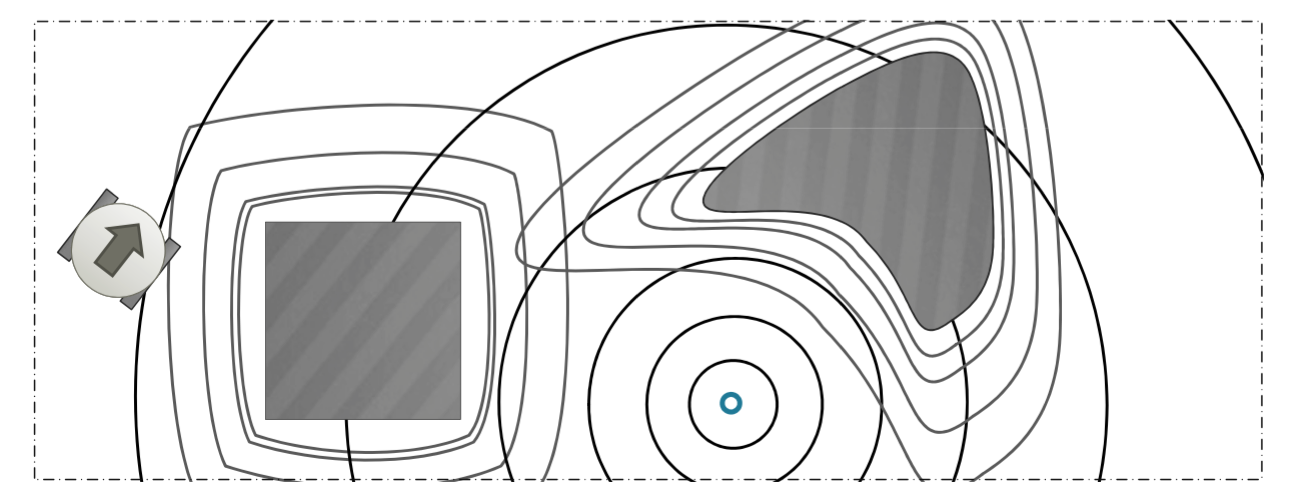
\includegraphics[width=0.75\textwidth]{images/pot_field.png}
   \caption{Potential field method working principle \citep{siegwart2004autonomous}. Grey areas represent obstacles, the blue circle represents a goal. Depicted in grey and black lines are the equipotential lines of the repulsive and attractive potentials respectively. The robot will follow the direction of the largest gradient, based on his starting position.} 
   \label{pics:pot_field}
\end{figure}

The main limitation to this approach is that it is prone to local minima, where the robot can get stuck. However, we are not working with any goals, but rather with an user input in form of a force so even if the robot is within a local minima, the user can literally pull it away from it. Furthermore, because the output of the potential field method is a force vector, we can elegantly combine it with the admittance controller, which also operates using virtual forces acting on the robot. 

So we can conclude that the potential field method is most suitable for a fusion with an admittance controller and we will elaborate on our implementation in the following.

\chapter{Implementation}
\begin{figure}
   \centering
   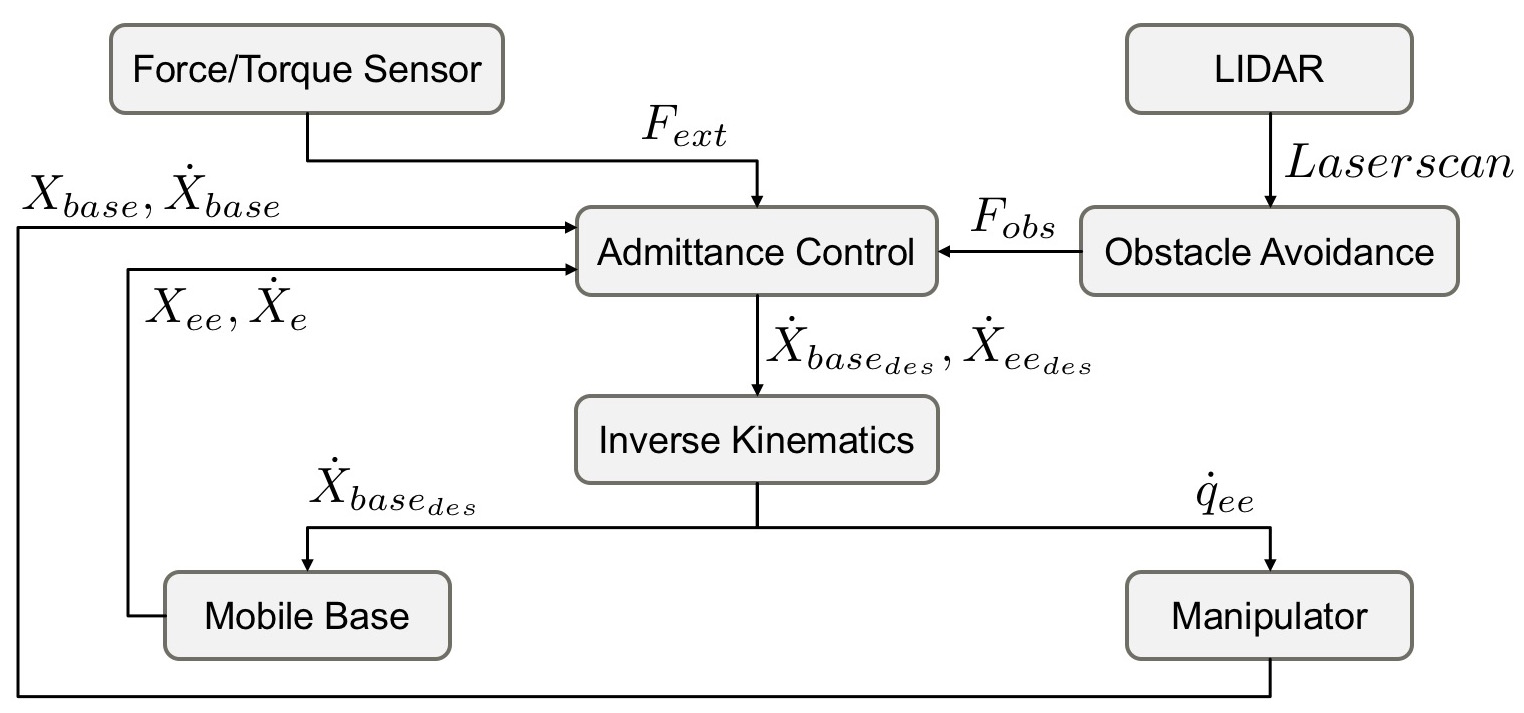
\includegraphics[width=0.75\textwidth]{images/controller_overview.jpg}
   \caption{Schematic of the controller. Boxes filled in grey are the nodes of the controller and the arrows indicate information flow between the nodes of the control architecture. The top level nodes are the sensor inputs, which are the readings from the \emph{force-torque sensor} and the \emph{LIDAR}. Beneath, we have the nodes which make up the controller, namely the \emph{admittance control}, the \emph{obstacle avoidance} and the \emph{inverse kinematics}. Nodes on the bottom represent the harwarde interfaces for the \emph{mobile base} and the \emph{manipulator}.}
   \label{pics:controller_overview}
\end{figure}

Having the potential field method selected as the desired obstacle avoidance algorithm, we can move on to fusing it together with the admittance controller. Figure \ref{pics:controller_overview} shows the overall controller schematic as a flowchart, with the nodes used and their messages exchanged, and Table \ref{tab:controller_nodes} summarizes the individual nodes and their ROS messages used.

Firstly, we outline the overall functionality of the system by explaining the functionality of all nodes briefly and dive more deeply into nodes of interest subsequently.

\begin{description}
  \item[Force-torque sensor] The force-torque sensor node continuously outputs the readings from the FT300 (Chapter \ref{sec:ft300}) as a wrench $F_{ext}$ of dimension $\mathbb{R}^{6 \times 1}$. The top three elements are the linear force readings in $[N]$ and the latter the angular torque readings in $[Nm]$. All packed in a ROS message of type \emph{WrenchStamped} \citep{rosWrench} and published at a rate of \unit[100]{Hz}. 
  \item[LIDAR] The output of the LIDAR node are the scans from the Hokuyo laser range finder. Each \emph{LaserScan} ROS message \citep{rosLaserscan} contains the range and intensity of every laser measurement taken from the minimum to the maximum angle of the sensor.
  \item[Obstacle avoidance] Given the laserscan readings, the obstacle avoidance node creates a costmap \citep{rosCostmap} around the mobile manipulator, which is explained in detail in Chapter \ref{sec:costmap}. The costmap is the obstacle potential of all obstacles seen in the laserscans and we derive the resulting force $F_{obs}$ analogously to Equation \ref{eq:pot_force} as
  \begin{equation}
  F_(obs) = - \nabla U_{obs}(q)
  \end{equation}
  
  Because the costmap is in two dimensional horizontal space, the resulting force $F_{obs}$ is also planar and has dimension $\mathbb{R}^{2 \times 1}$. 
  
  \item[Admittance control] We feed these into the \emph{admittance control}, whose other inputs are the vehicle kinematics, namely the current pose $X_{base}$ \citep{rosPose} and twist $\dot{X}_{base}$ \citep{rosTwist} of the ridgeback \emph{mobile base} and the current pose $X_{ee}$ and twist $\dot{X}_{ee}$ of the UR10 \emph{manipulator}. Given these inputs, we calculate the desired twist $\dot{X}_{base_{des}}$ for the mobile base and the desired twist $\dot{X}_{ee_{des}}$ for the manipulator in cartesian space.
  
  \item[Inverse kinematics] which in terms needs to be put through the \emph{inverse kinematics} to obtain a feasible velocity $\dot{q}_{ee_{des}}$ in joint space for the manipulator.
  \item[Mobile base] This node represents the hardware interface and the low level controller of the Ridgeback. It accepts a command velocity as input and using the wheel odometry, it can accurately estimate its pose $X_{base}$ and velocity $\dot{X}_{base}$ and publish these.
  \item[Manipulator] This node represents the hardware interface and the low level controller of the UR10. Joint command inputs can be given through a FollowJointTrajectory action server \citep{rosJointTrajectory}, to which we continuously publish the command joint positions $q_{ee_{des}}$. Similarly to the mobile base node, outputs are the pose $X_{ee}$ and velocity $\dot{X}_{ee}$.
\end{description}

\begin{table}[h]
\begin{center}
 \caption{Controller nodes and their respective outputs.}\vspace{1ex}
 \label{tab:controller_nodes}
 \begin{tabular}{l|lccl}
 \hline
Node & Output & Dimension & Unit & ROS message type \\ \hline \hline
Force-torque sensor & $F_{ext}$ & $\mathbb{R}^{6 \times 1}$ & $[N]$ & WrenchStamped \\
LIDAR & $F_{obs}$ & $\mathbb{R}^{2 \times 1}$ & $[N]$ & WrenchStamped \\
Admittance control & $\dot{X}_{base},\dot{X}_{ee}$ & $\mathbb{R}^{10 \times 1}$ & $[N]$ & Custom twist message \\
Inverse kinematics & $\dot{X}_{base_{des}}$ & $\mathbb{R}^{3 \times 1}$  & $[\sfrac{m}{s}]$ & TwistStamped \\
& $\dot{q}_{ee_{des}}$&$\mathbb{R}^{6 \times 1}$ & $[rad]$ & FollowJointTrajectory\\
Mobile base & $X_{base}$ & $\mathbb{R}^{7 \times 1}$ & $[m]$ & PoseStamped \\
& $\dot{X}_{base}$ & $\mathbb{R}^{6 \times 1}$ & $[\sfrac{m}{s}]$ & TwistStamped \\
Manipulator & $X_{ee}$ & $\mathbb{R}^{7 \times 1}$ & $[m]$ & PoseStamped \\
& $\dot{X}_{ee}$ & $\mathbb{R}^{6 \times 1}$ & $[\sfrac{m}{s}]$ & TwistStamped \\


 \hline
 \end{tabular}
\end{center}
\end{table}

\section{Admittance Control and Obstacle Avoidance Fusion}
\begin{figure}
   \centering
   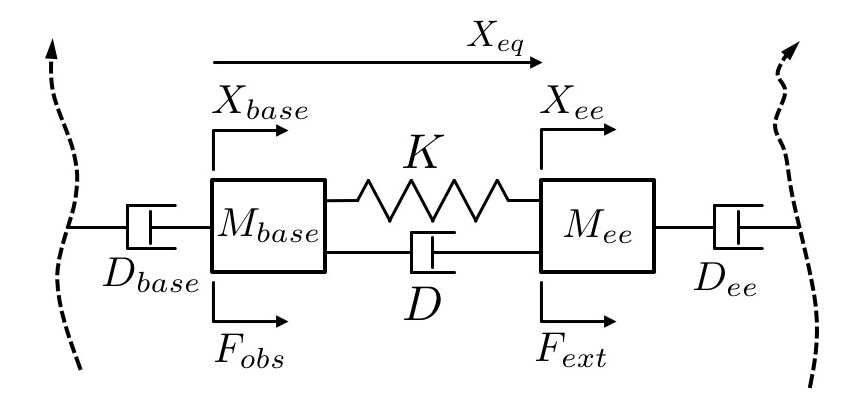
\includegraphics[width=0.75\textwidth]{images/admittance_model.jpg}
   \caption{Virtual spring mass damper system with two masses. Dotted arrows represent the path of the base (left) and the arm (right) over time, connected by the spring mass damper system.}
   \label{pics:admittance_model}
\end{figure}
The key element of the whole algorithm is the fusion of the admittance controller, as described in Chapter \ref{sec:adm_ctrl} and the obstacle avoidance, as described in Chapter \ref{sec:pot_field}. In order to achieve this, we define a virtual two mass spring damper system, depicted in Figure \ref{pics:admittance_model}. Here $M_{ee}$ represents the virtual mass of the EE with pose $X_{ee}$ and $M_{base}$ the virtual mass of the Ridgeback with pose $X_{base}$. We couple the two masses together using a spring element with a spring constant $K$ and a damping element with a damping constant $D$. This coupling has an equilibrium position which is defined a priori and is denoted by $X_{eq}$. As the name suggests,  the coupling is in an equilibrium when

\begin{equation}
\overline{\rm X_{base}X_{ee}} = X_{eq}
\end{equation}

Furthermore, we add additional damping elements $D_{ee}$ and $D_{base}$, through which we couple the two masses to their desired trajectories, depicted as dotted arrows in Figure \ref{pics:admittance_model}.

Since the EE is where the system is connected to the human partner, any external force $F_{ext}$ exerted by him attacks at $M_{ee}$. Similarly, because the Ridgeback is running the obstacle avoidance, any force $F_{obs}$ created by it has to attack at $M_{base}$ in the system. 

Applying Equation \ref{eq:mass_spring_damper_sys} to both rigid elements in our virtual system yields the control equations of the fused admittance control and obstacle avoidance algorithm

\begin{equation}
M_{base} \cdot \ddot{X}_{base} = -D_{base} \cdot \dot{X}_{base} - D \cdot \dot{X}_{ee} + K \cdot X_{error}+F_{obs}
	\label{eq:adm_base}
\end{equation}

\begin{equation}
M_{ee} \cdot \ddot{X}_{ee} = -(D + D_{ee}) \cdot \dot{X}_{ee} - K \cdot X_{error}+F_{ext}
	\label{eq:adm_ee}
\end{equation}

where $X_{error}$ is the deviation from the equilibrium pose $X_{eq}$

\begin{equation}
X_{error} = \overline{\rm X_{base}X_{ee}} - X_{eq}
\end{equation}

where Equation \ref{eq:adm_base} is the force equilibrium for the Ridgeback and Equation \ref{eq:adm_ee} the force equilibrium for the EE. We can see that through this coupling, any force $F_{ext}$ exerted by the human parter on the EE will also result in a velocity response of the Ridgeback and vice versa will any obstacle force $F_{obs}$ also result in a velocity response of the EE.

\subsection{Control Parameters}
In this chapter, we list and elaborate on the tuned parameters used in Equation \ref{eq:adm_base} and \ref{eq:adm_ee}. Since we are in six dimensional space and we are not interested in having any interdependence between the individual axes, all constants are six dimensional diagonal matrices. Therefore, we guarantee a full decoupling of all axes.

We set the equilibrium pose $X_eq$ of the EE in respect to the frame of the armbase to be offset by \unit[1]{m} in $x$ and \unit[0.5]{m} in $z$. Equation \ref{eq:eq_pose} shows the full pose in $\mathbb{R}^{7 \times 1}$, consisting of a position and a quaternion\footnote{The UR10 base frame is rotated by \unit[180]{$\degree$} around the vertical axis $z$ in respect to the Ridgeback base frame, hence the negative sign in $x$.}.
\begin{equation}
X_{eq} = \begin{pmatrix}
-1 \\ 0 \\ 0.5 \\ 0 \\ 0 \\ 0.7071067 \\ 0.7071069 \\
\end{pmatrix} \begin{bmatrix}
m \\
- \\
\end{bmatrix}
	\label{eq:eq_pose}
\end{equation}

Since all our parameters are virtual, we can start off by setting the mass of the EE $M_{ee}$ as the identity matrix. From there, we tune the remaining parameters $M_{base}$, $D_{ee}$,$D_{base}$,$D$ and $K$, which is essentially the same as tuning a PID controller. The goal is to have a fast response on the EE, so that jerky input from the human partner can be compensated and a slower response by the Ridgeback to follow the overall trajectory.

\begin{equation}
M_{ee} = \begin{pmatrix}
1 & 0 & 0 & 0 & 0 & 0 \\
0 & 1 & 0 & 0 & 0 & 0 \\
0 & 0 & 1 & 0 & 0 & 0 \\
0 & 0 & 0 & 1 & 0 & 0 \\
0 & 0 & 0 & 0 & 1 & 0 \\
0 & 0 & 0 & 0 & 0 & 1 \\
\end{pmatrix}
\begin{bmatrix}
kg \\
kg \cdot m^2 \\
\end{bmatrix}
\end{equation}

\begin{equation}
D_{ee} = \begin{pmatrix}
8 & 0 & 0 & 0 & 0 & 0 \\
0 & 8 & 0 & 0 & 0 & 0 \\
0 & 0 & 8 & 0 & 0 & 0 \\
0 & 0 & 0 & 20 & 0 & 0 \\
0 & 0 & 0 & 0 & 20 & 0 \\
0 & 0 & 0 & 0 & 0 & 8 \\
\end{pmatrix}
\begin{bmatrix}
\frac{N s}{m} \\
N m s
\end{bmatrix}
\end{equation}

An important note here is that although Equation \ref{eq:adm_base} is six dimensional, the output sent to the Ridgeback is only three dimensional, as explained in Chapter \ref{sec:ridgeback}. Hence, parameters in linear $z$, angular $x$ and angular $y$, i.e., the third through fifth rows of Equation \ref{eq:M_base} and Equation \ref{eq:D_base} are irrelevant for the performance of the controller.

\begin{equation}
M_{base} = \begin{pmatrix}
0.1 & 0 & 0 & 0 & 0 & 0 \\
0 & 0.1 & 0 & 0 & 0 & 0 \\
0 & 0 & 10 & 0 & 0 & 0 \\
0 & 0 & 0 & 10 & 0 & 0 \\
0 & 0 & 0 & 0 & 10 & 0 \\
0 & 0 & 0 & 0 & 0 & 0.1 \\
\end{pmatrix}
\begin{bmatrix}
kg \\
kg \cdot m^2 \\
\end{bmatrix}
\label{eq:M_base}
\end{equation}

\begin{equation}
D_{base} = \begin{pmatrix}
20 & 0 & 0 & 0 & 0 & 0 \\
0 & 10 & 0 & 0 & 0 & 0 \\
0 & 0 & 0 & 0 & 0 & 0 \\
0 & 0 & 0 & 0 & 0 & 0 \\
0 & 0 & 0 & 0 & 0 & 0 \\
0 & 0 & 0 & 0 & 0 & 4 \\
\end{pmatrix}
\begin{bmatrix}
\frac{N s}{m} \\
N m s
\end{bmatrix}
\label{eq:D_base}
\end{equation}

\begin{equation}
D = \begin{pmatrix}
0 & 0 & 0 & 0 & 0 & 0 \\
0 & 0 & 0 & 0 & 0 & 0 \\
0 & 0 & 0 & 0 & 0 & 0 \\
0 & 0 & 0 & 0 & 0 & 0 \\
0 & 0 & 0 & 0 & 0 & 0 \\
0 & 0 & 0 & 0 & 0 & 0 \\
\end{pmatrix}
\begin{bmatrix}
\frac{N s}{m} \\
N m s
\end{bmatrix}
\end{equation}

We set the stiffness of the coupling in Equation \ref{eq:K} deliberately to \unitfrac[500]{N}{m} in linear $z$, because we want the jointly carried object to be close to the height of the equilibrium pose, independent of its weight. Similarly, we set the stiffness in angular $x$ and angular $y$ to \unit[500]{Nm}, in order to prevent rotation of the object around these two axes.

\begin{equation}
K = \begin{pmatrix}
150 & 0 & 0 & 0 & 0 & 0 \\
0 & 150 & 0 & 0 & 0 & 0 \\
0 & 0 & 500 & 0 & 0 & 0 \\
0 & 0 & 0 & 500 & 0 & 0 \\
0 & 0 & 0 & 0 & 500 & 0 \\
0 & 0 & 0 & 0 & 0 & 100 \\
\end{pmatrix}
\begin{bmatrix}
\frac{N}{m} \\
N m
\end{bmatrix}
\label{eq:K}
\end{equation}

\subsection{Costmap of the Obstacle Potential}
	\label{sec:costmap}
	
Using the ROS costmap package \citep{rosCostmap}, this node builds a two dimensional occupancy grid based on the incoming laserscans and inflates the cost according to user specified parameters. Table \ref{tab:costmap_params} lists all parameters and their set values. Since we do only local planning, a local costmap, meaning the center of the costmap is equal to the center of the robot, of size \unit[3 $\times$ 3]{m} suffices.

The algorithm assigns a value from 0 to 100 to every cell of the occupancy grid, which represents the cost $c$ of that cell. We can distinguish four types of cells:

\begin{description}
  \item[Lethal] A lethal cost is assigned to all cells, which are currently occupied by an obstacle and would therefore guarantee a collision, if the robot center would be at one of these cells.
  \begin{equation}
  c_{lethal} = 100
  \end{equation}
  \item[Inscribed] This category applies to all cells, whose distance to an obstacle is less than the radius of the robot, which is defined by the parameter \emph{robot footprint}. Similarly to the lethal cells, a collision is guaranteed if the robot center overlaps with an inscribed cell.
    \begin{equation}
  c_{inscribed} = 99
  \end{equation}
  \item[Obstacle proximity] Obstacle proximity groups all cells, that make up the repulsive potential $U_{rep}$ of the obstacle, as defined in Equation \ref{eq:pot_field_repulsive}. The distance threshold \emph{inflation radius} defines the size of the potential and the \emph{inflater layer cost scaling factor} defines the steepness of the quadratic curve. These cells represent that the robot center is close to an obstacle but not necessarily colliding.
    \begin{equation}
  c_{proximity} = \begin{bmatrix}
  1,98 \\ 
  \end{bmatrix}
  \end{equation}
  \item[Freespace] All cells that are further away from an obstacle than the distance threshold \emph{inflation radius} are set to 0, meaning that the robot can travel freely through theses cells.
    \begin{equation}
  c_{free} = 0
  \end{equation}
\end{description}

Figure \ref{pics:costmap} depicts an example of the costmap of a scenario, where the Thing is between two obstacles.

\begin{figure}
   \centering
   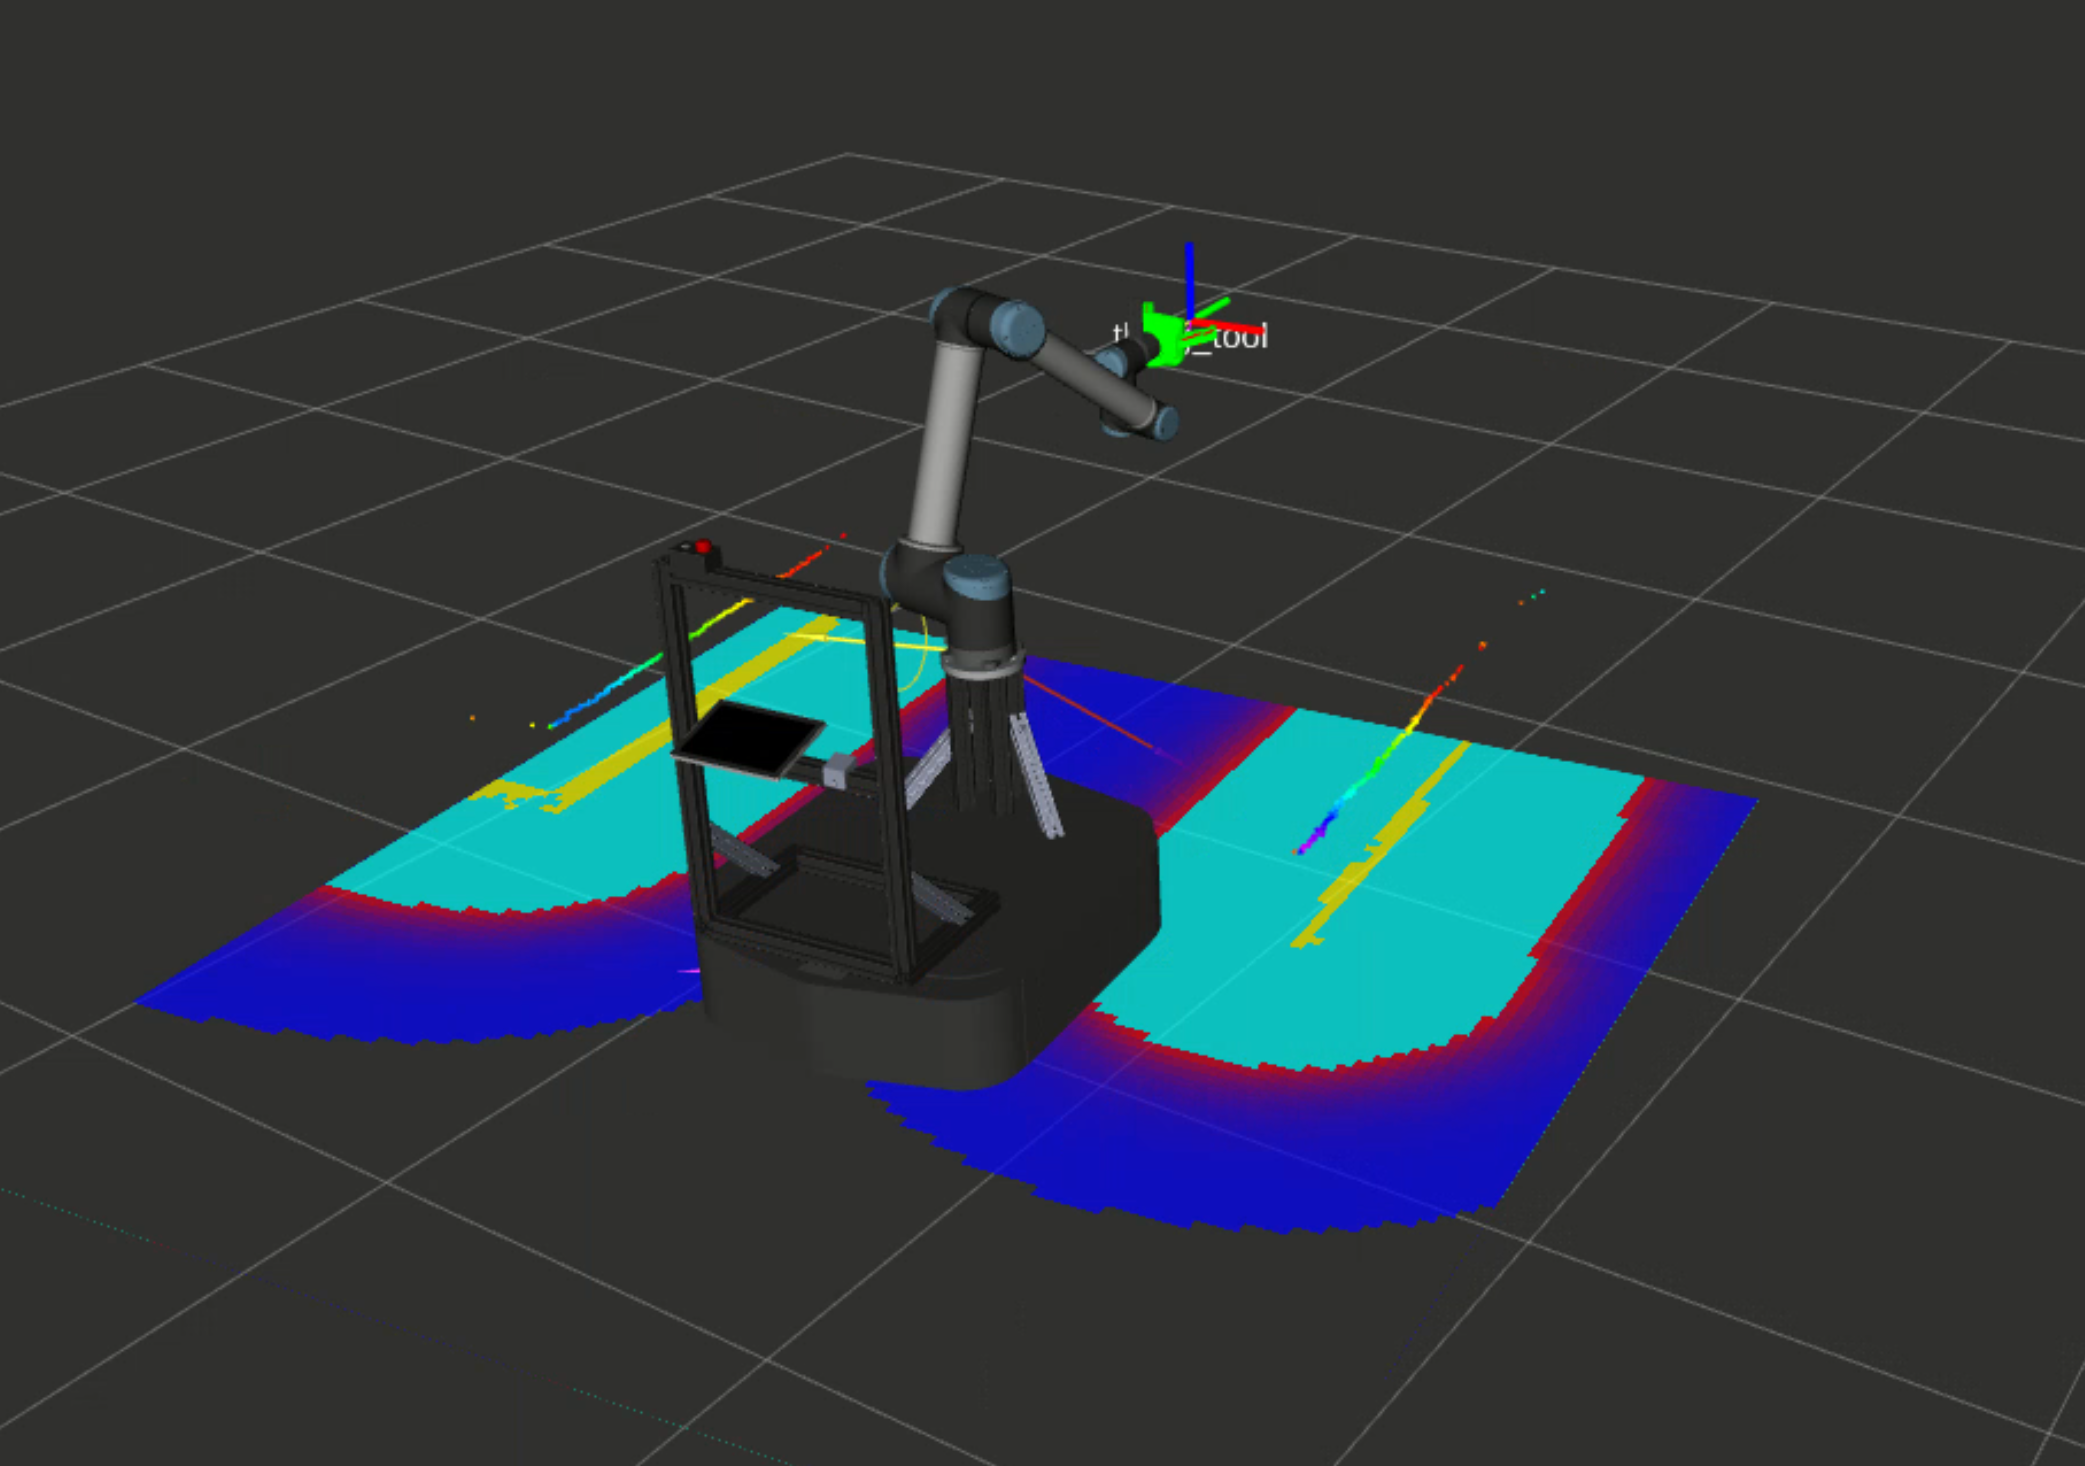
\includegraphics[width=0.75\textwidth]{images/costmap.png}
   \caption{Costmap visualization during a test, depicted with the simulation of the Thing.  \textsc{Yellow:} Lethal cells ($c = 100$), \textsc{Turquoise:} Inscribed cells ($c = 99$), \textsc{Red to Blue gradient:} Proximity to an obstacle ($c = [1,98]$), \textsc{Transparent:} Free space ($c = 0$).}
   \label{pics:costmap}
\end{figure}

\begin{table}[h]
\begin{center}
 \caption{Costmap Parameters.}\vspace{1ex}
 \label{tab:costmap_params}
 \begin{tabular}{ll}
 \hline
Type & Local \\
Update frequency & \unit{60}{Hz} \\
Publish frequency & \unit{60}{Hz} \\ 
Width & \unit{3}{m} \\
Height & \unit{3}{m} \\
Resolution & \unit{0.03}{m} \\
Global frame & Base link \\
Static map & False \\
Rolling window & True \\
Robot footprint & \unit{0.96 $\times$ 0.8}{m} \\
Plugins used & Obstacles layer, inflater layer \\
Inflater layer cost scaling factor & 10  \\
Inflation radius & \unit{2}{m} \\
 \hline
 \end{tabular}
\end{center}
\end{table}

\section{Task Priority Inverse Kinematics}
Forward kinematics, which is the mapping from joint coordinates $q$ to the end-effector configuration $X_{ee}$ of a mobile manipulator, is a well understood problem and can be solved using the \emph{Jacobian} $J(q)$ which is defined as

\begin{equation}
J(q) =
\begin{bmatrix}
\frac{\partial X_1}{\partial q_1} & \hdots & \frac{\partial X_1}{\partial q_{n_j}} \\
\vdots & \ddots & \vdots \\
\frac{\partial X_m}{\partial q_1} & \hdots & \frac{\partial X_m}{\partial q_{n_j}}
\end{bmatrix}
\end{equation}

It relates differences from joint coordinates $q$ to EE configuration  space $X_{ee}$:

\begin{equation}
\dot{X}_{ee} = J(q) \cdot \dot{q}
\end{equation}

The inverse kinematics, i.e., the calculation of the joint velocity $\dot{q}$ given an EE velocity $\dot{X}_{ee}$ is already trickier, but can be achieved using the \emph{Moore-Penrose pseudo inverse} $J^+$ of the Jacobian:

\begin{equation}
\dot{q} = J^+ \cdot \dot{X}_{ee} 
\end{equation}

where $J^+$ is defined as

\begin{equation}
J^+ = J^T(JJ^T)^{-1}
\end{equation}

Furthermore, because we are working with a mobile manipulator and not a rigidly fixed robot arm, there are two cartesian velocities $\dot{X}_1$ and $\dot{X}_2$, for which we want to solve simultaneously. Hence, we use a multi-task inverse kinematics control that can prioritize among multiple tasks \citep{nakamura1987task}. This is achieved by utilizing \emph{null-space optimization} to execute a secondary task with Jacobian $J_2$, given a primary task with Jacobian $J_1$.

\begin{equation}
\dot{q} = J_1^+ \dot{X}_1 + N_1 J_2^+ N_1 (\dot{X}_2-J_2J_1^+\dot{X}_1)
\label{eq:task_priority}
\end{equation}

Equation \ref{eq:task_priority} formulates the task priority approach to inverse kinematics for two tasks, with $N_i$ being the null-space projection matrix of $J_i$, fulfilling the condition

\begin{equation}
J_i N_i = 0
\end{equation}

The simplest projection is given by
\begin{equation}
N_i = \mathbb{I} - J_i^+J_i
\end{equation}
where $\mathbb{I}$ denotes the identity matrix.

Since an accurate execution of the desired Ridgeback velocity $\dot{X}_{base_{des}}$ is crucial to ensure a successful obstacle avoidance, we choose $\dot{X}_{base_{des}}$ to be our primary task and $\dot{X}_{ee_{des}}$ our secondary.

\chapter{Results}
We test our previously elaborated implementation on the Thing and list the performed tests and their results in this chapter. Figure \ref{pics:test_setup} depicts the test setup of the Thing gripping the object to be jointly carried. The object is made from wood and \unit[91.44]{cm} in length. Furthermore, we have all low level controllers running on the computer embedded in the Ridgeback and the admittance control and obstacle avoidance running on a laptop, connected through Ethernet.


\begin{figure}[h]
   \centering
   \includegraphics[width=0.75\textwidth]{images/test_setup.jpg}
   \caption{The Thing holding the jointly carried object used in the tests. It is a wooden structure \unit[3]{feet} or \unit[91.44]{cm} in length and equipped with a handle to facilitate gripping.}
   \label{pics:test_setup}
\end{figure}

\section{Admittance Control Performance}
	\label{sec:adm_ctrl_performance}
As initial tests, we analyse the behaviour of the admittance controller in isolation. For this, we place the Thing in free space with no obstacles, i.e., in a region with zero gradient and excite three axes separately by applying force and torque on the object. The three axes are linear $x$, linear $y$ and angular $z$, i.e., the three DOF of the Ridgeback. Therefore, we see a response of both the base and the end-effector in all three tests.

Figure \ref{pics:test18_x} depicts the velocity response of the system to a force excitement in $x$, Figure \ref{pics:test18_y} the response to a force excitement in $y$ and Figure \ref{pics:test18_theta} around $z$, i.e., the angular velocity $\theta$ given a torque input around $z$.

\begin{figure}
   \centering
   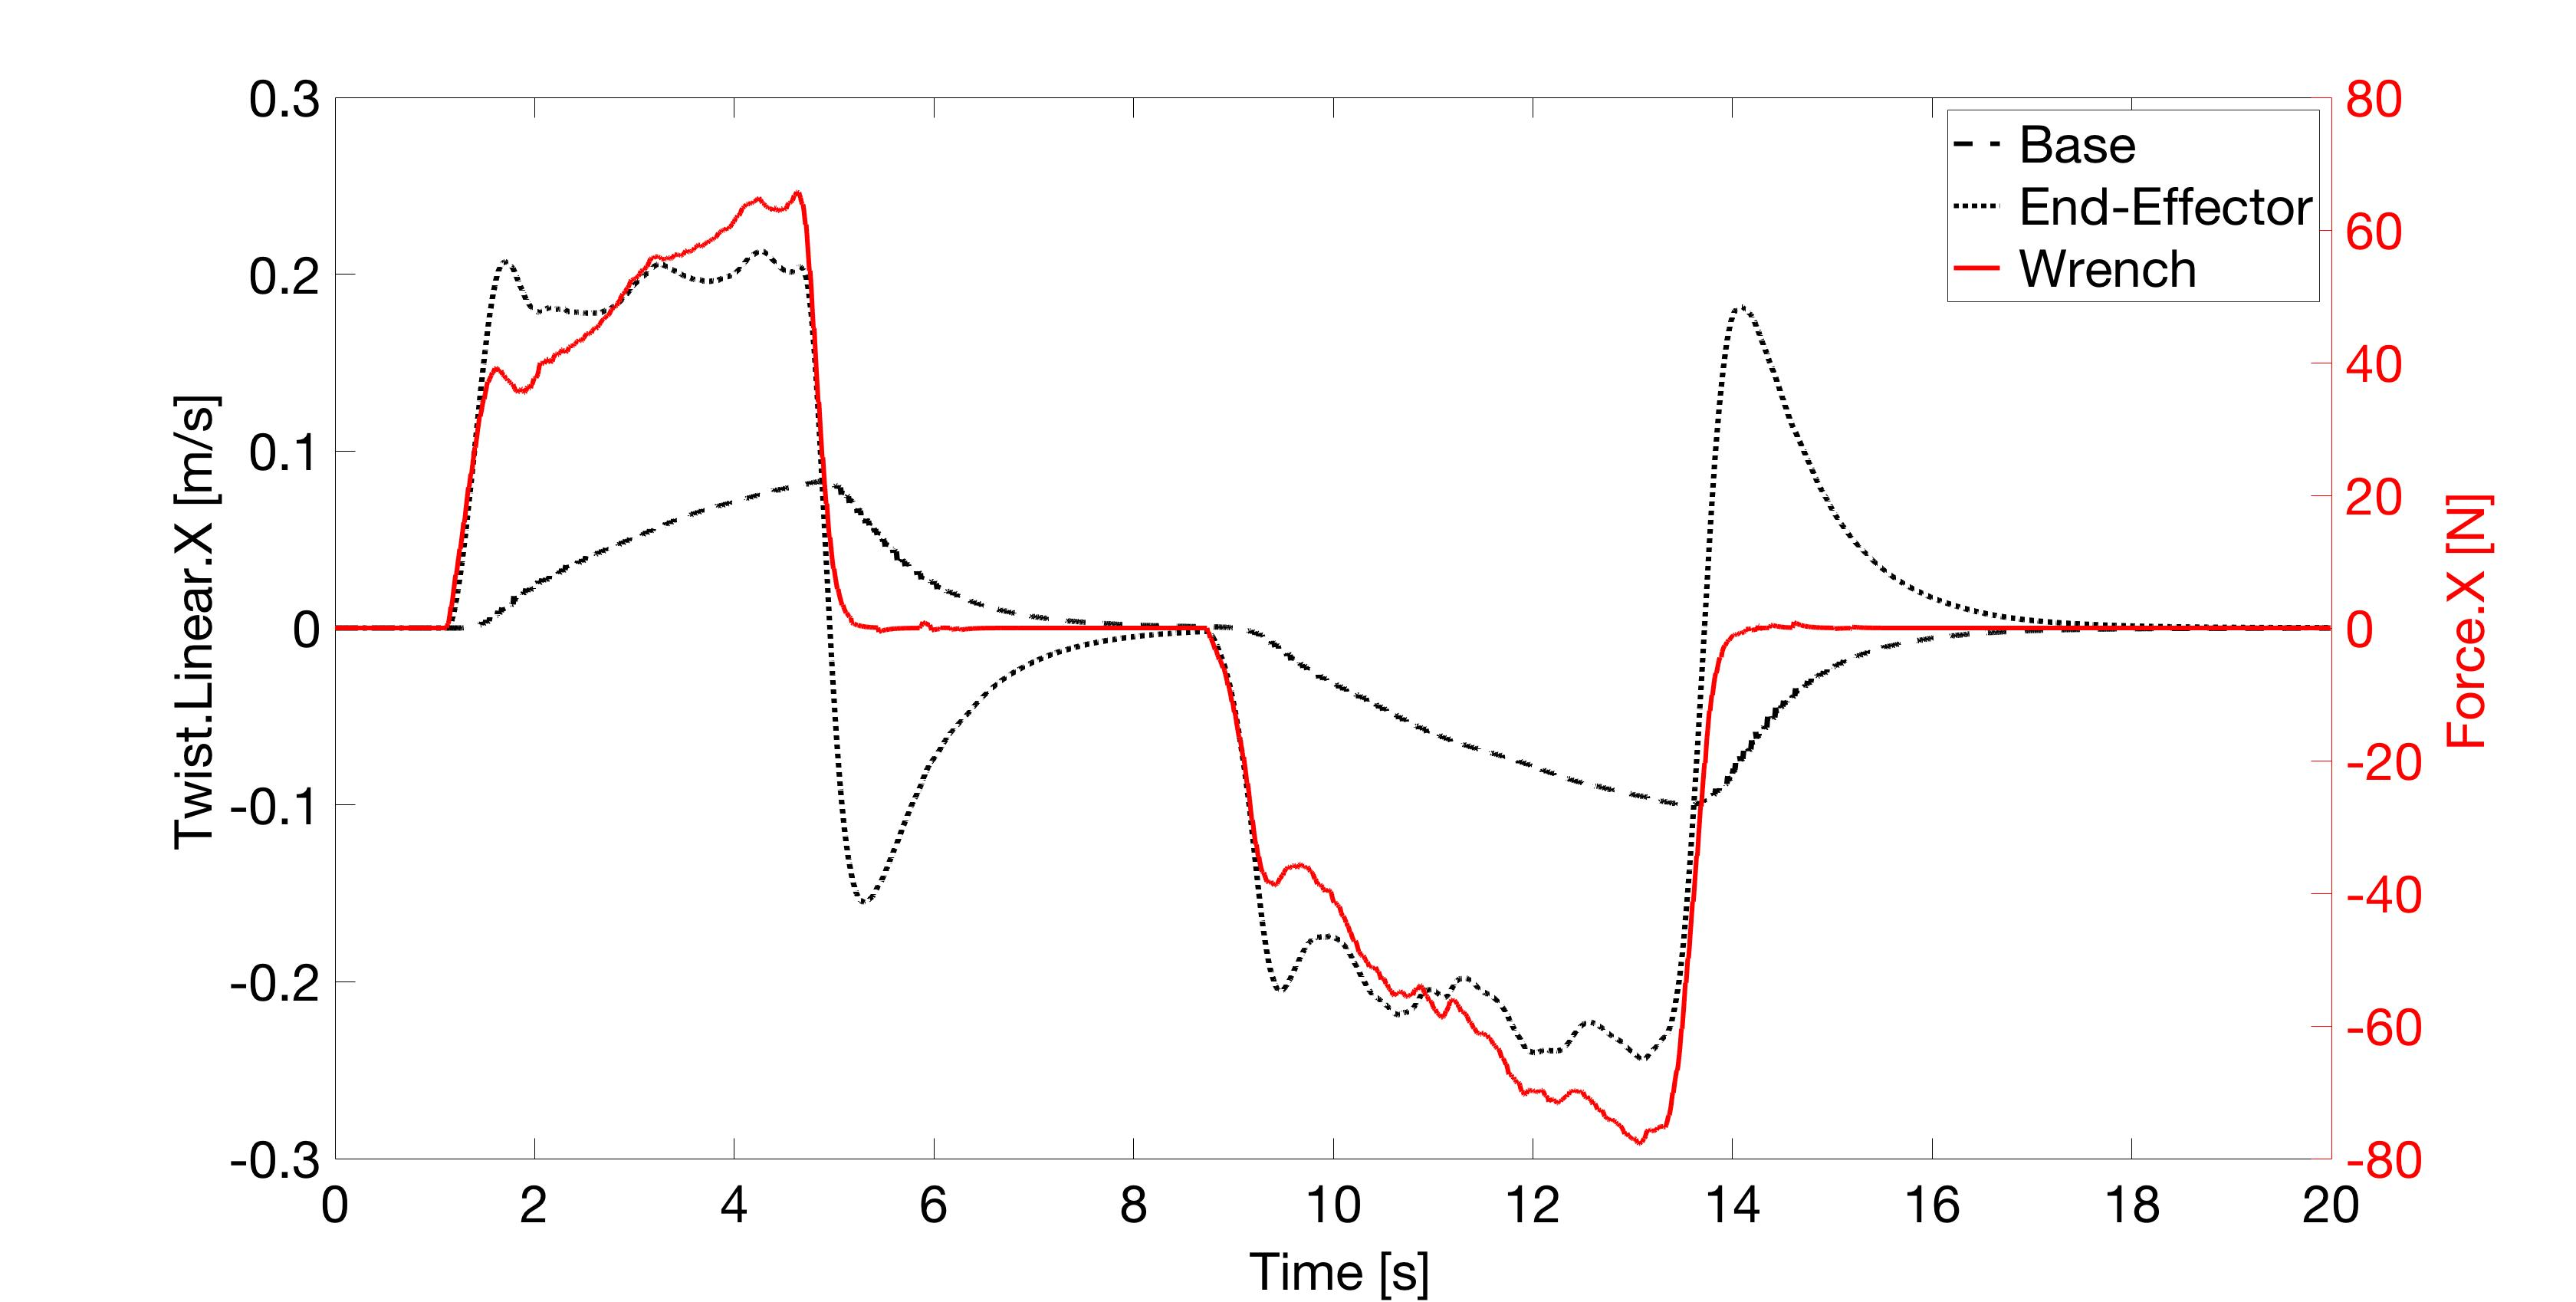
\includegraphics[width=0.75\textwidth]{images/test18_x.jpg}
   \caption{Velocity Response to Force Excitement in $x$}
   \label{pics:test18_x}
\end{figure}

\begin{figure}
   \centering
   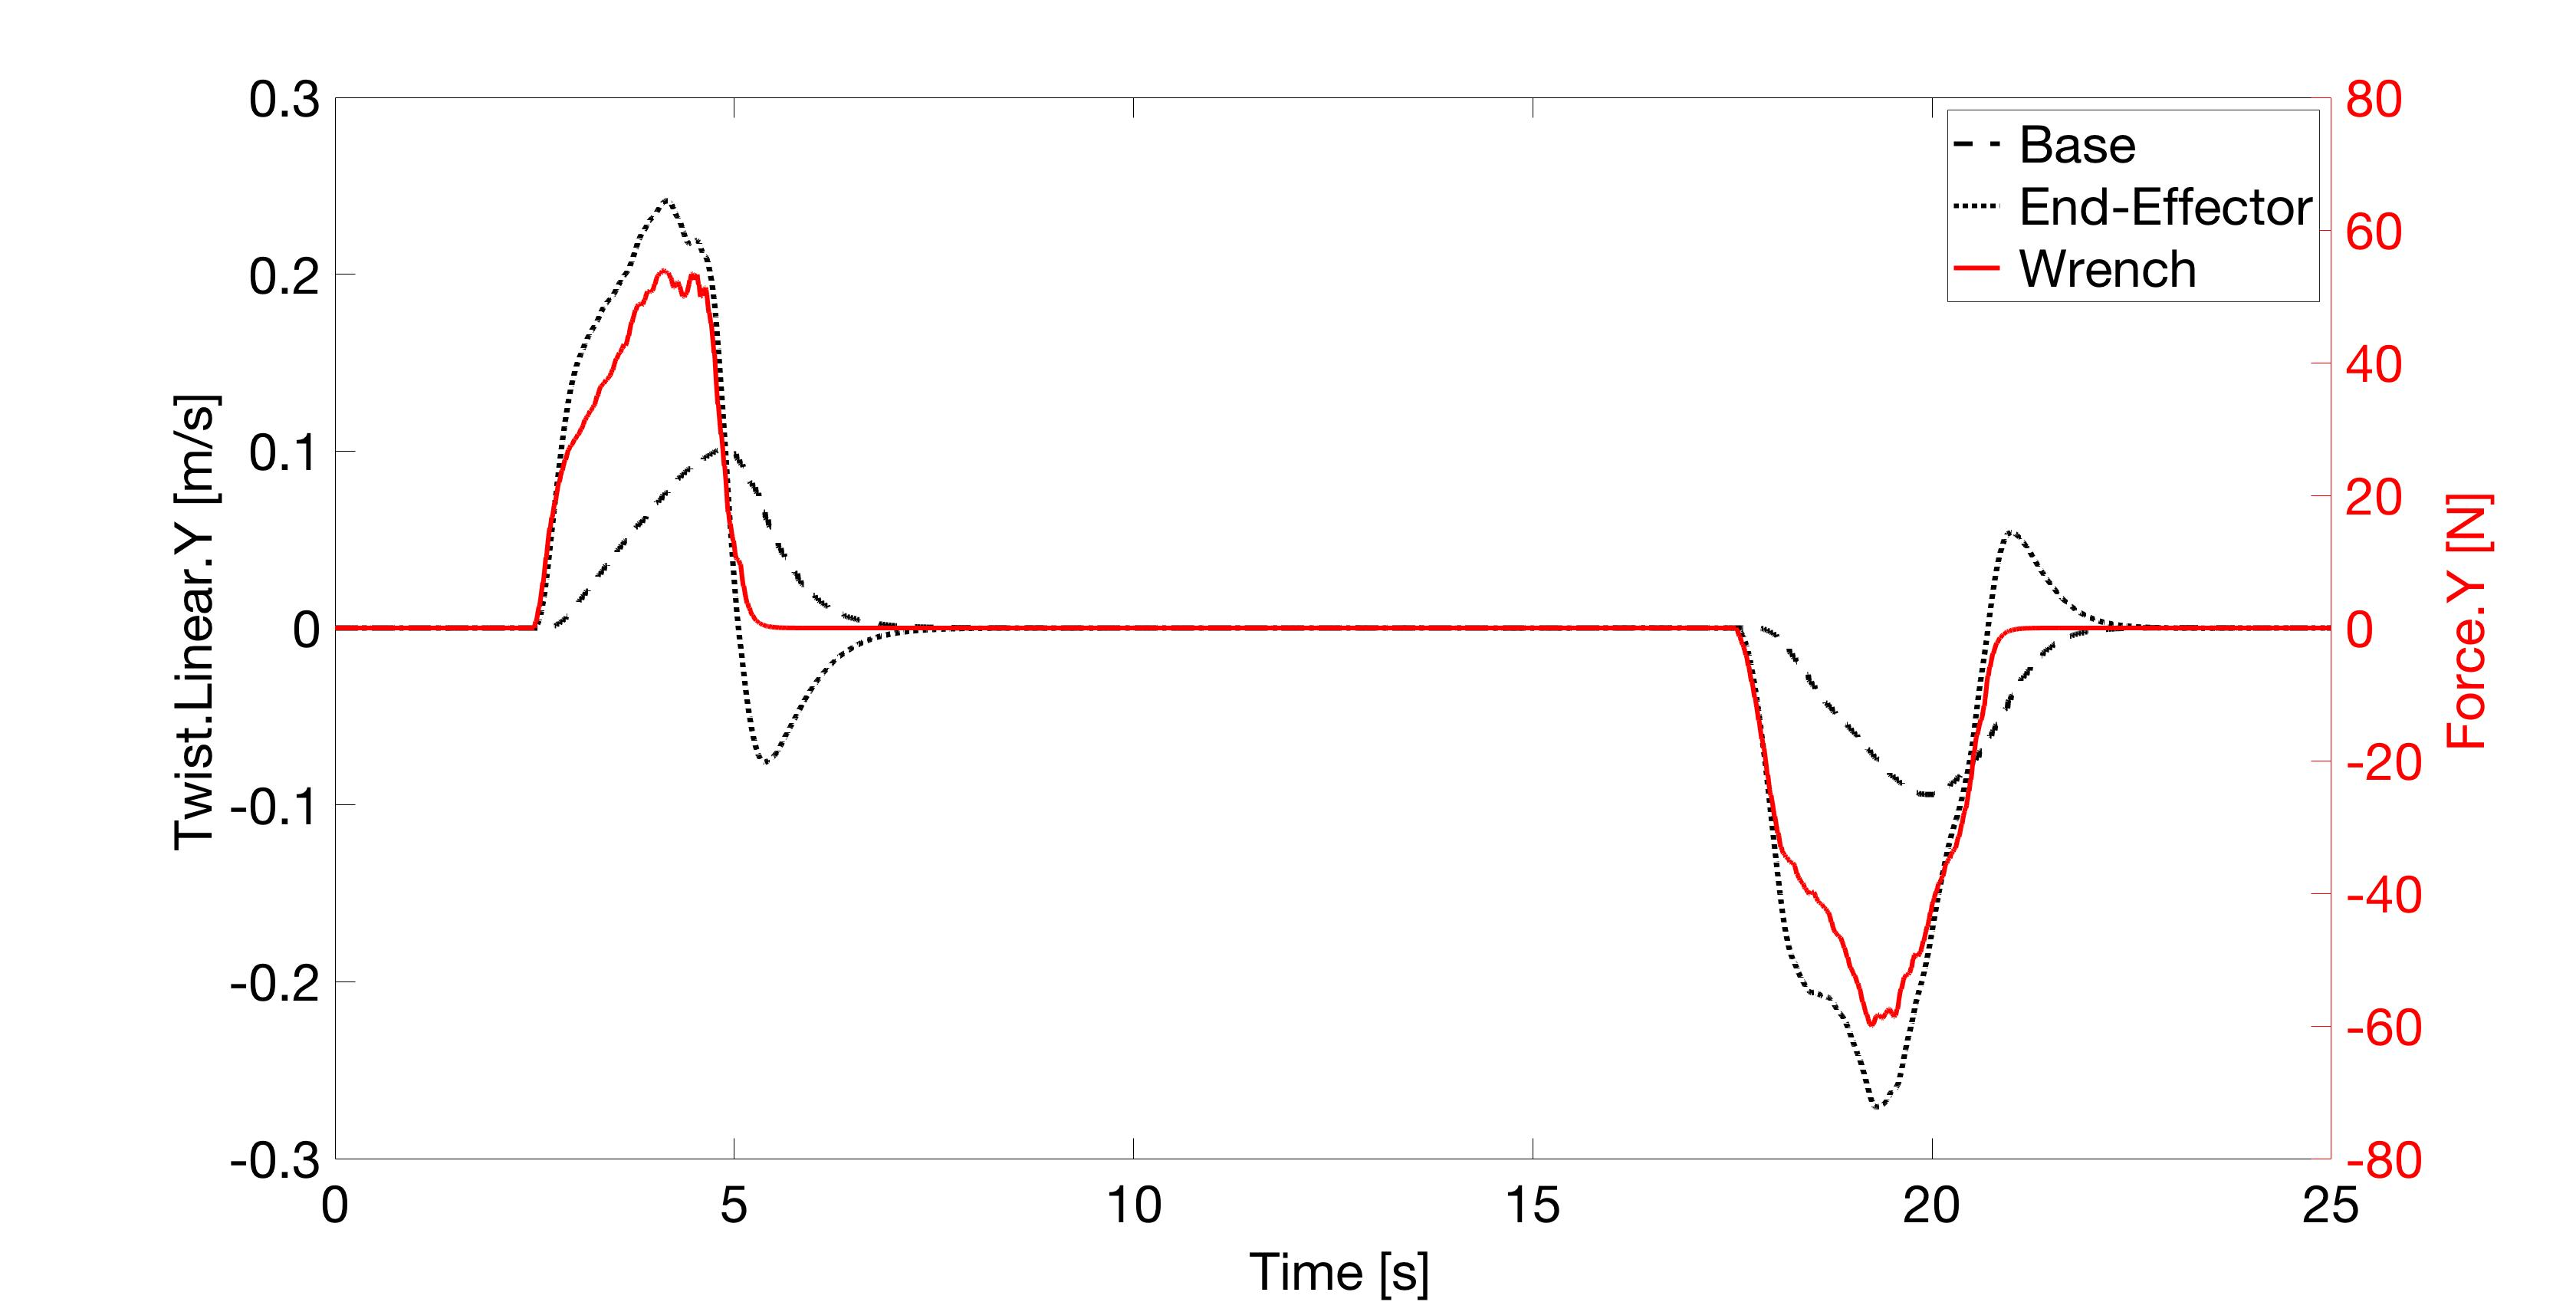
\includegraphics[width=0.75\textwidth]{images/test18_y.jpg}
   \caption{Velocity Response to Force Excitement in $y$}
   \label{pics:test18_y}
\end{figure}

\begin{figure}
   \centering
   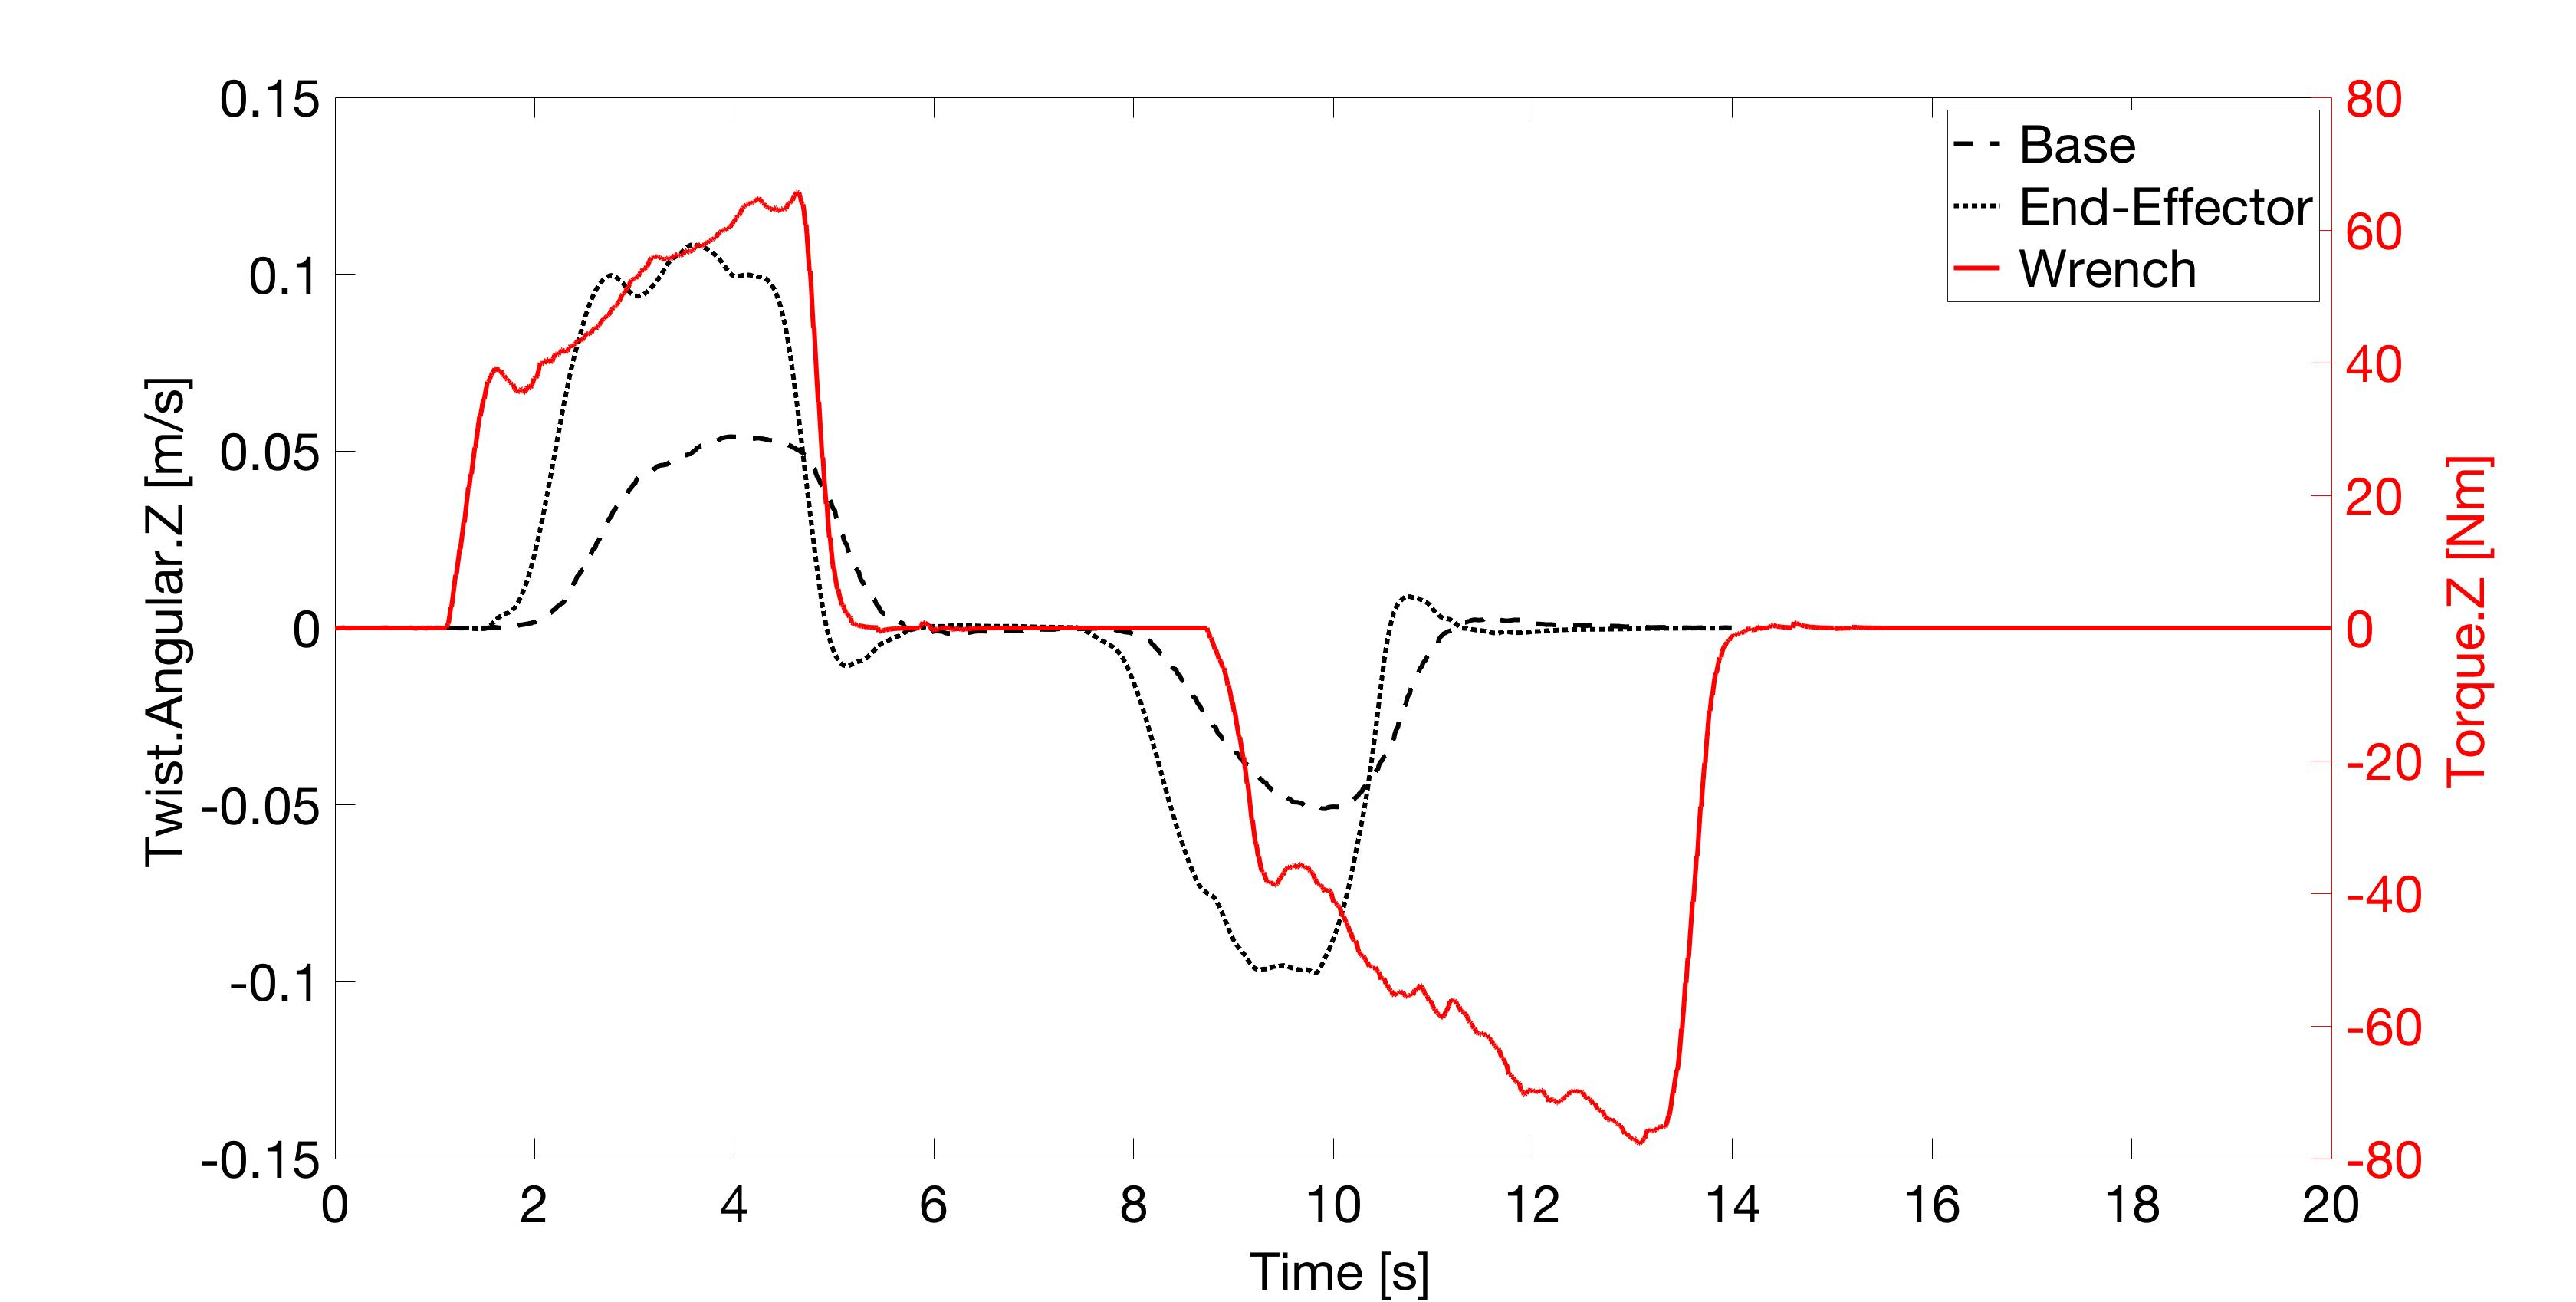
\includegraphics[width=0.75\textwidth]{images/test18_theta.jpg}
   \caption{Velocity Response to Torque Excitement around $z$}
   \label{pics:test18_theta}
\end{figure}

If we look at the response of the EE in both $x$, $y$ and $\theta$, we notice that it has a under-critically damped controller, which leads to a quick rise time and overshooting in the opposite direction, as soon as no more force is applied. This behaviour is actually desired, since we want to counteract sudden movement and jerky input by the human partner with the EE and only output smooth behaviour to the Ridgeback. If we have a look at the velocity response in $x$, $y$ and $\theta$ of the latter, we see a vastly slower rise time and no overshooting, i.e., a critically damped controller.

Furthermore, we notice that the linear velocity response of the EE peaks at \unitfrac[0.2]{m}{s} and the linear velocity response of the Ridgeback at \unitfrac[0.1]{m}{s}.

\section{Obstacle Avoidance and Admittance Control Performance}
Having the admittance controller tuned and working as desired, we can move on to testing the full algorithm where obstacle avoidance comes into play. We use cardboard boxes of dimension \unit[14 $\times$ 14 $\times$ 60]{inches} as obstacles, so that in case of a failure of the controller and an occurrence of a crash, the Thing does not get damaged.

Because we have no \unit[360]{\degree} \textsf{Lidar} coverage, but only a front-facing field of view, we can test the obstacle avoidance in forward and sideways motion of the Thing only. However, we've seen in Chapter \ref{sec:adm_ctrl_performance}, that the response to the admittance controller is independent of direction. Hence, we can assume that the full algorithm is scalable to a backward motion as well, if a back-facing \textsf{Lidar} were to be mounted.

\subsection{Frontal Obstacle}
The first obstacle avoidance test is the robot being pulled into a obstacle directly ahead of him. The scenario is depicted in Figure \ref{pics:test2_setup}. The velocity response of the system in the direction of pull, which is $x$, is plotted in Figure \ref{pics:test2}.

\begin{figure}[h]
   \centering
   \includegraphics[width=0.75\textwidth]{images/test2_setup.jpg}
   \caption{Set up of the frontal obstacle test scenario.}
   \label{pics:test2_setup}
\end{figure}

We see that the velocity responses of both EE and Ridgeback are constant, if a constant force is applied by the human partner and no obstacle is in range. However, as soon as we close in on the obstacle, the obstacle force pointing away from the obstacle rises and gradually diminishes the velocity respones to zero, although there is still a constant external force applied.

Figure \ref{pics:test2_costmap} depicts the cost map of the algorithm at the end of the experiment, i.e., at the robots closest position to the obstacle. We see the robot comes no closer than four grid cells to the obstacle, which equals a minimum obstacle clearance of \unit[12]{cm}. Together with the width of the Ridgeback of \unit[0.8]{m}, the lower bound on a narrow passage is thus slightly above\unit[1]{m}.

\begin{figure}
   \centering
   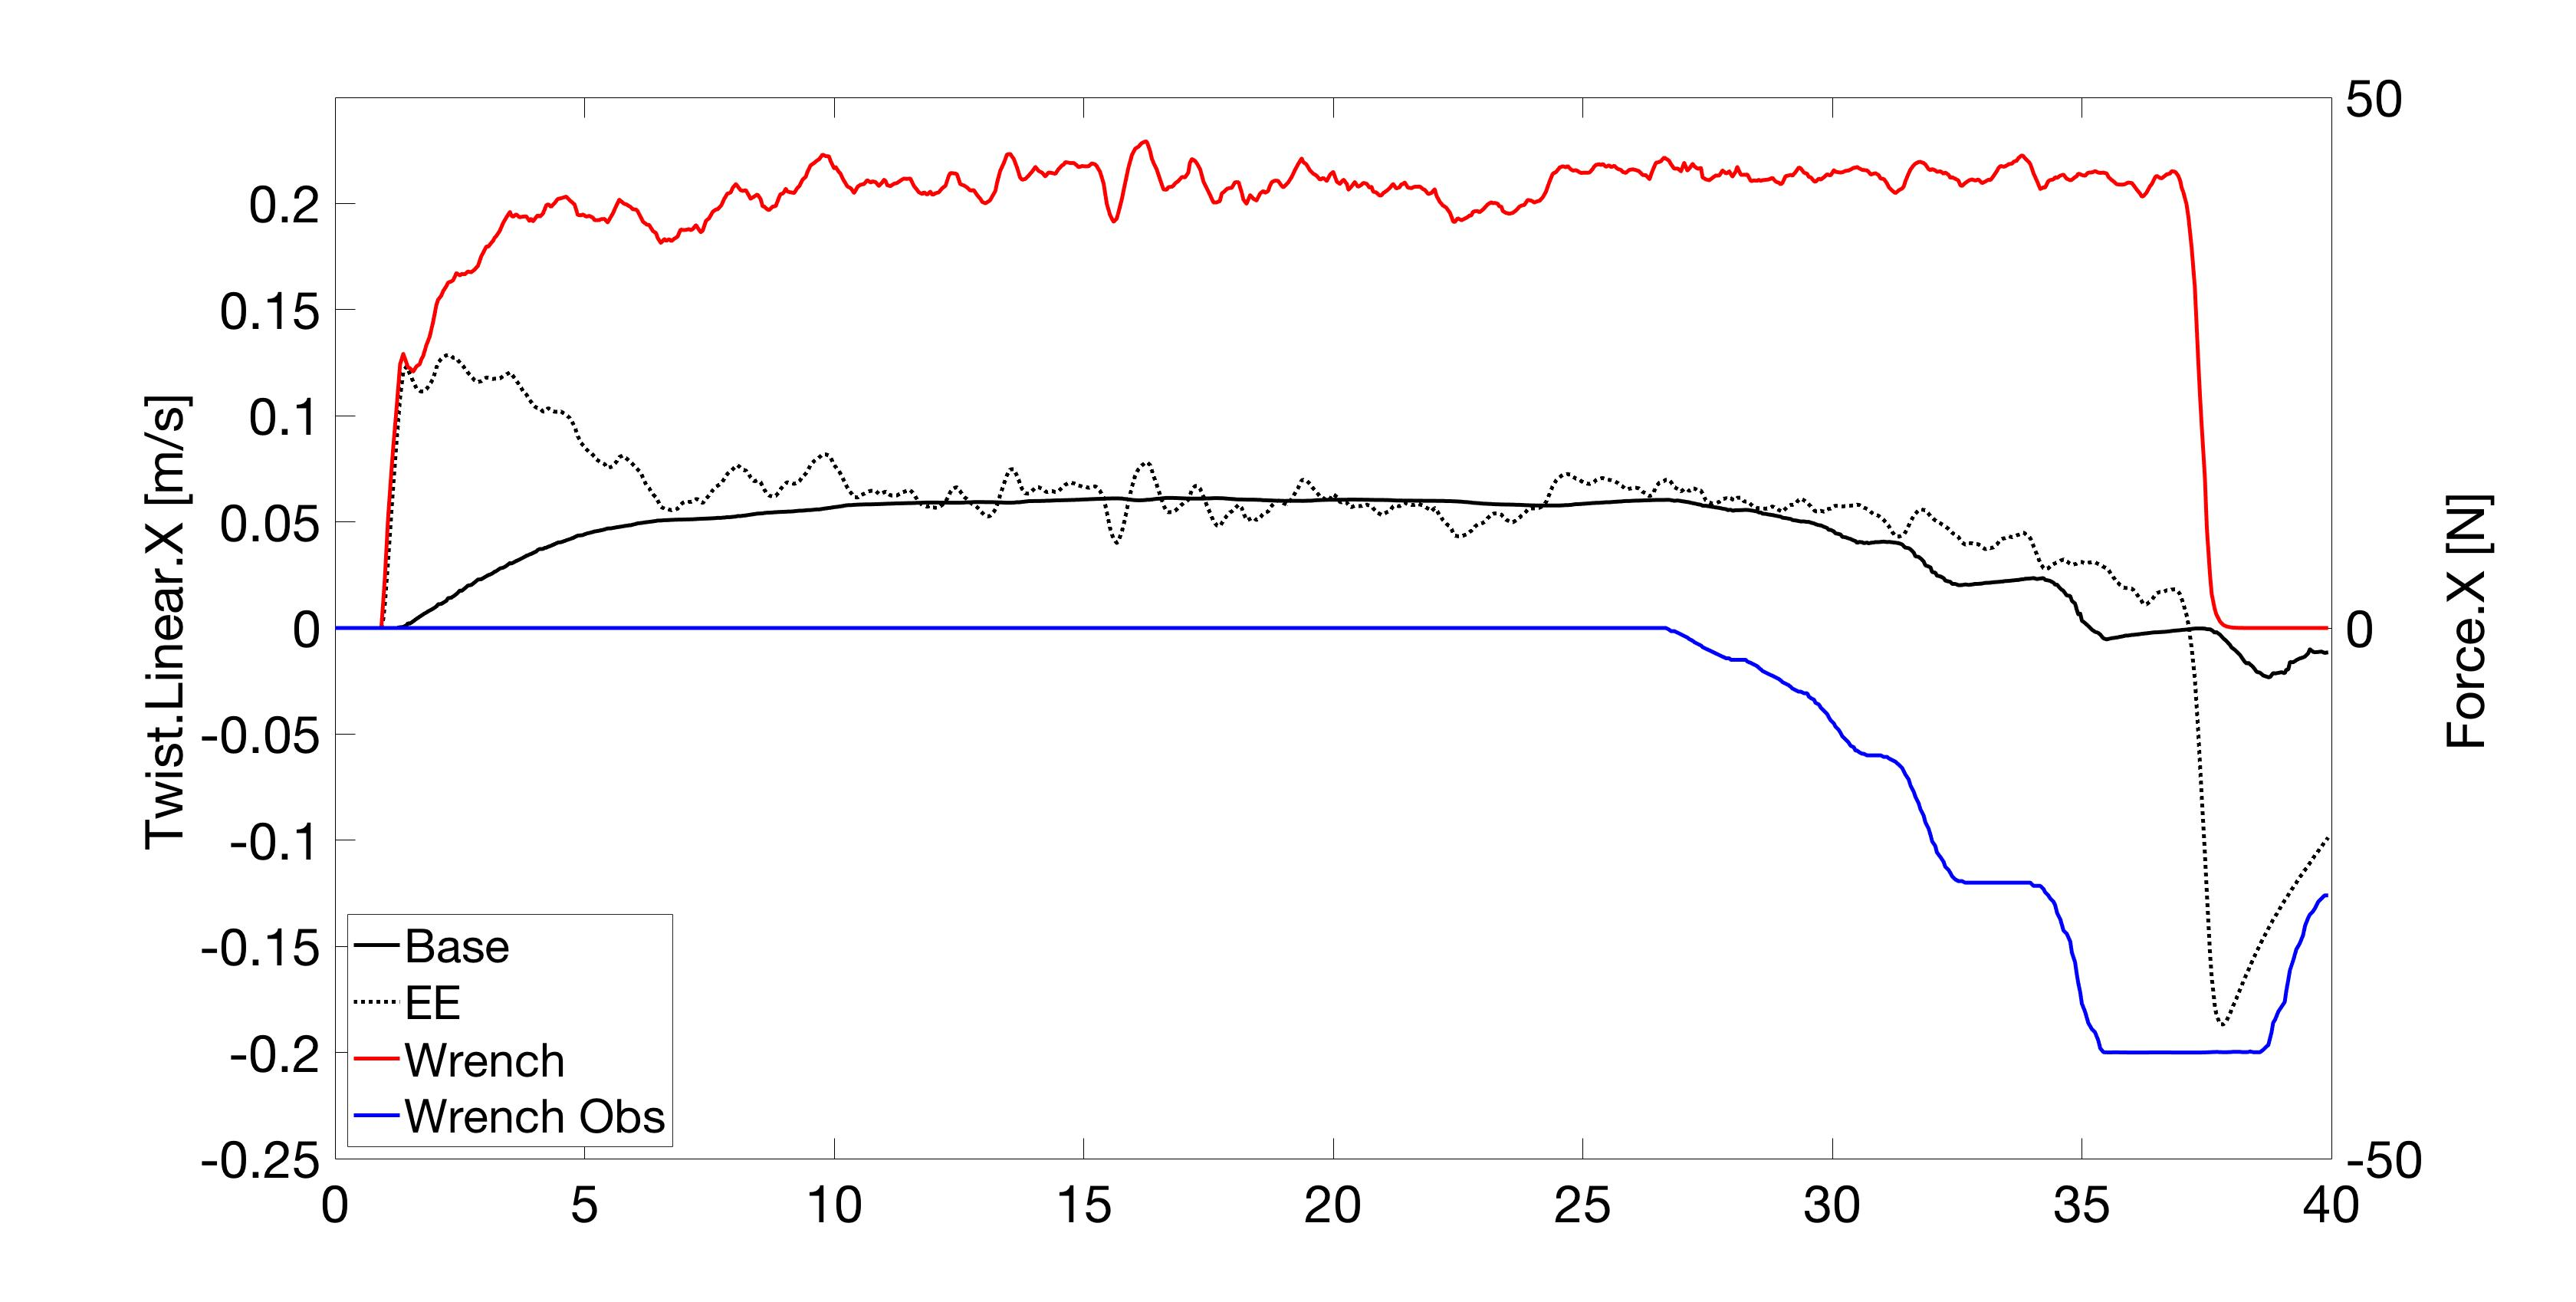
\includegraphics[width=0.75\textwidth]{images/test2.jpg}
   \caption{Velocity response in X axis of the robot to external and obstacle force input while being pulled in a frontal obstacle.}
   \label{pics:test2}
\end{figure}

\begin{figure}
   \centering
   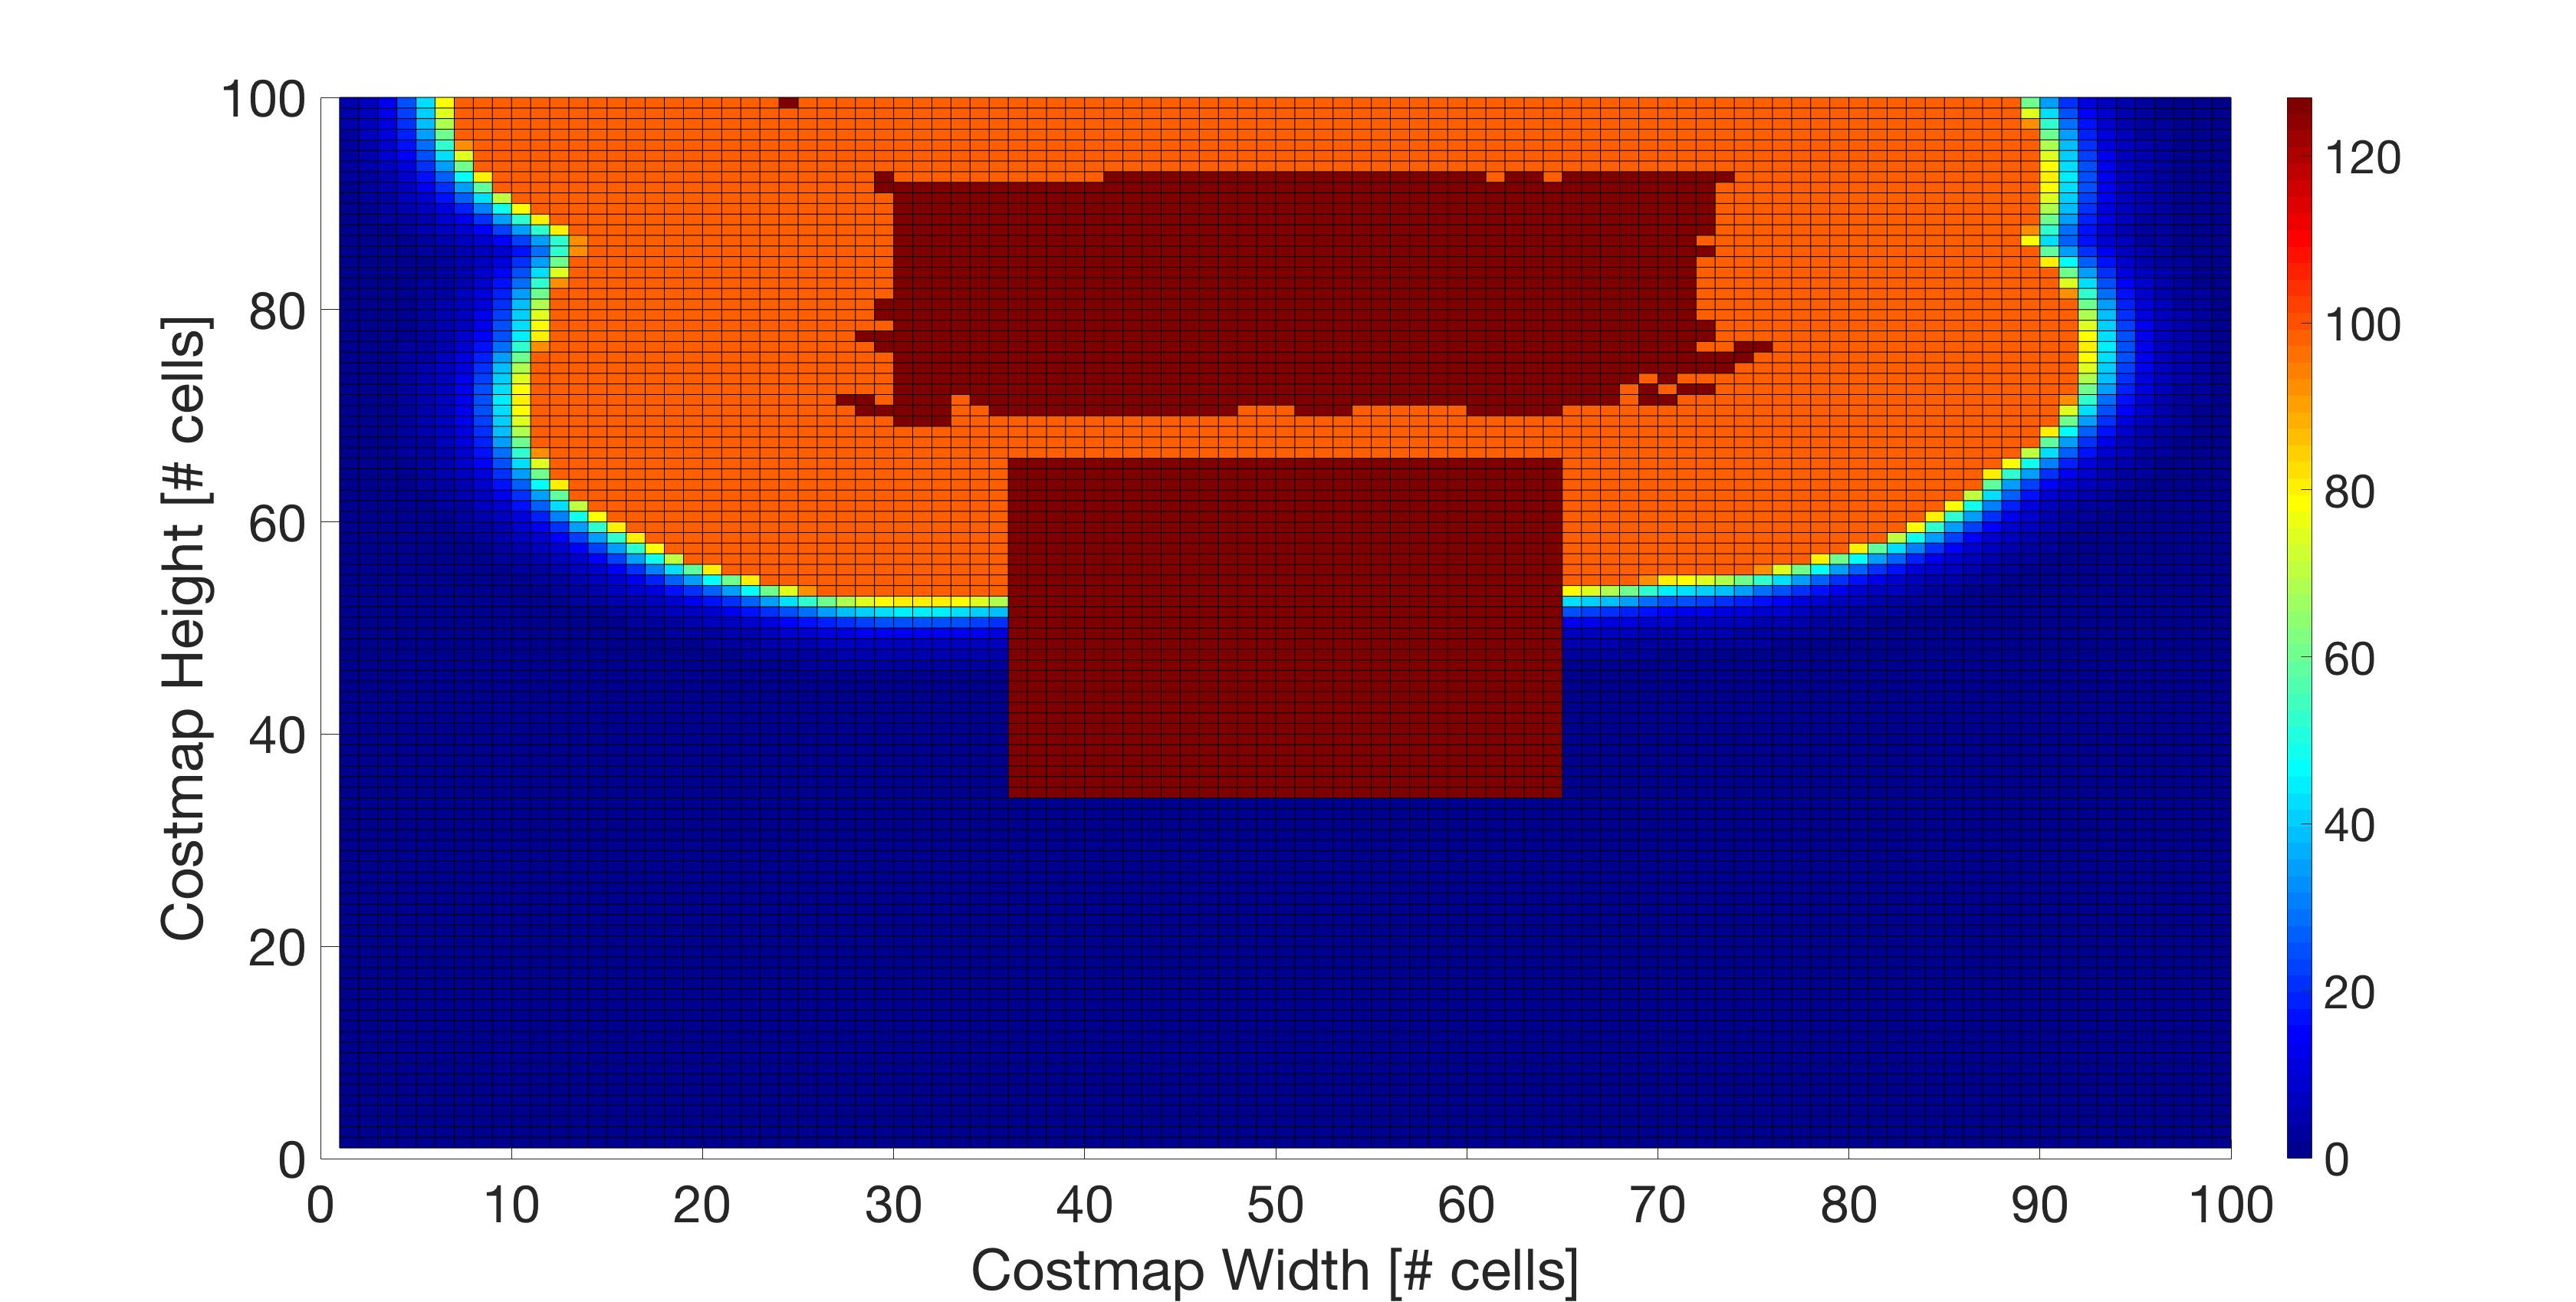
\includegraphics[width=0.75\textwidth]{images/test2_costmap.jpg}
   \caption{Costmap at \unit{34}{s} of the frontal test. Dark red indicate the obstacle and the robot base.}
   \label{pics:test2_costmap}
\end{figure}

\subsection{Corner}
In this experiment, we asses the performance of the algorithm in a corridor with a corner. The width of corridor is \unit{2}{m} and we jointly carry the object through it. The set-up at the beginning of the test is depicted in Figure \ref{pics:test16_setup}.

\begin{figure}[h]
   \centering
   \includegraphics[width=0.75\textwidth]{images/test16_setup2.jpg}
   \caption{Setup of the \unit{2}{m} wide corner scenario.}
   \label{pics:test16_setup}
\end{figure}

As we can see in Figure \ref{pics:test16}, there is a peak in the negative $y$ direction, which is caused by the robot drifting close to the outer wall as it is making the corner. This is due to the fact, that it is difficult for the human partner to apply torque in angular $z$, which makes the Thing rotate in place, without applying force in linear $y$, which makes the Thing move sideways. Hence, the trajectory of Ridgeback does not follow the center line of the hallway in a corner scenario, but rather utilizes the full width of the hallway.

\begin{figure}
   \centering
   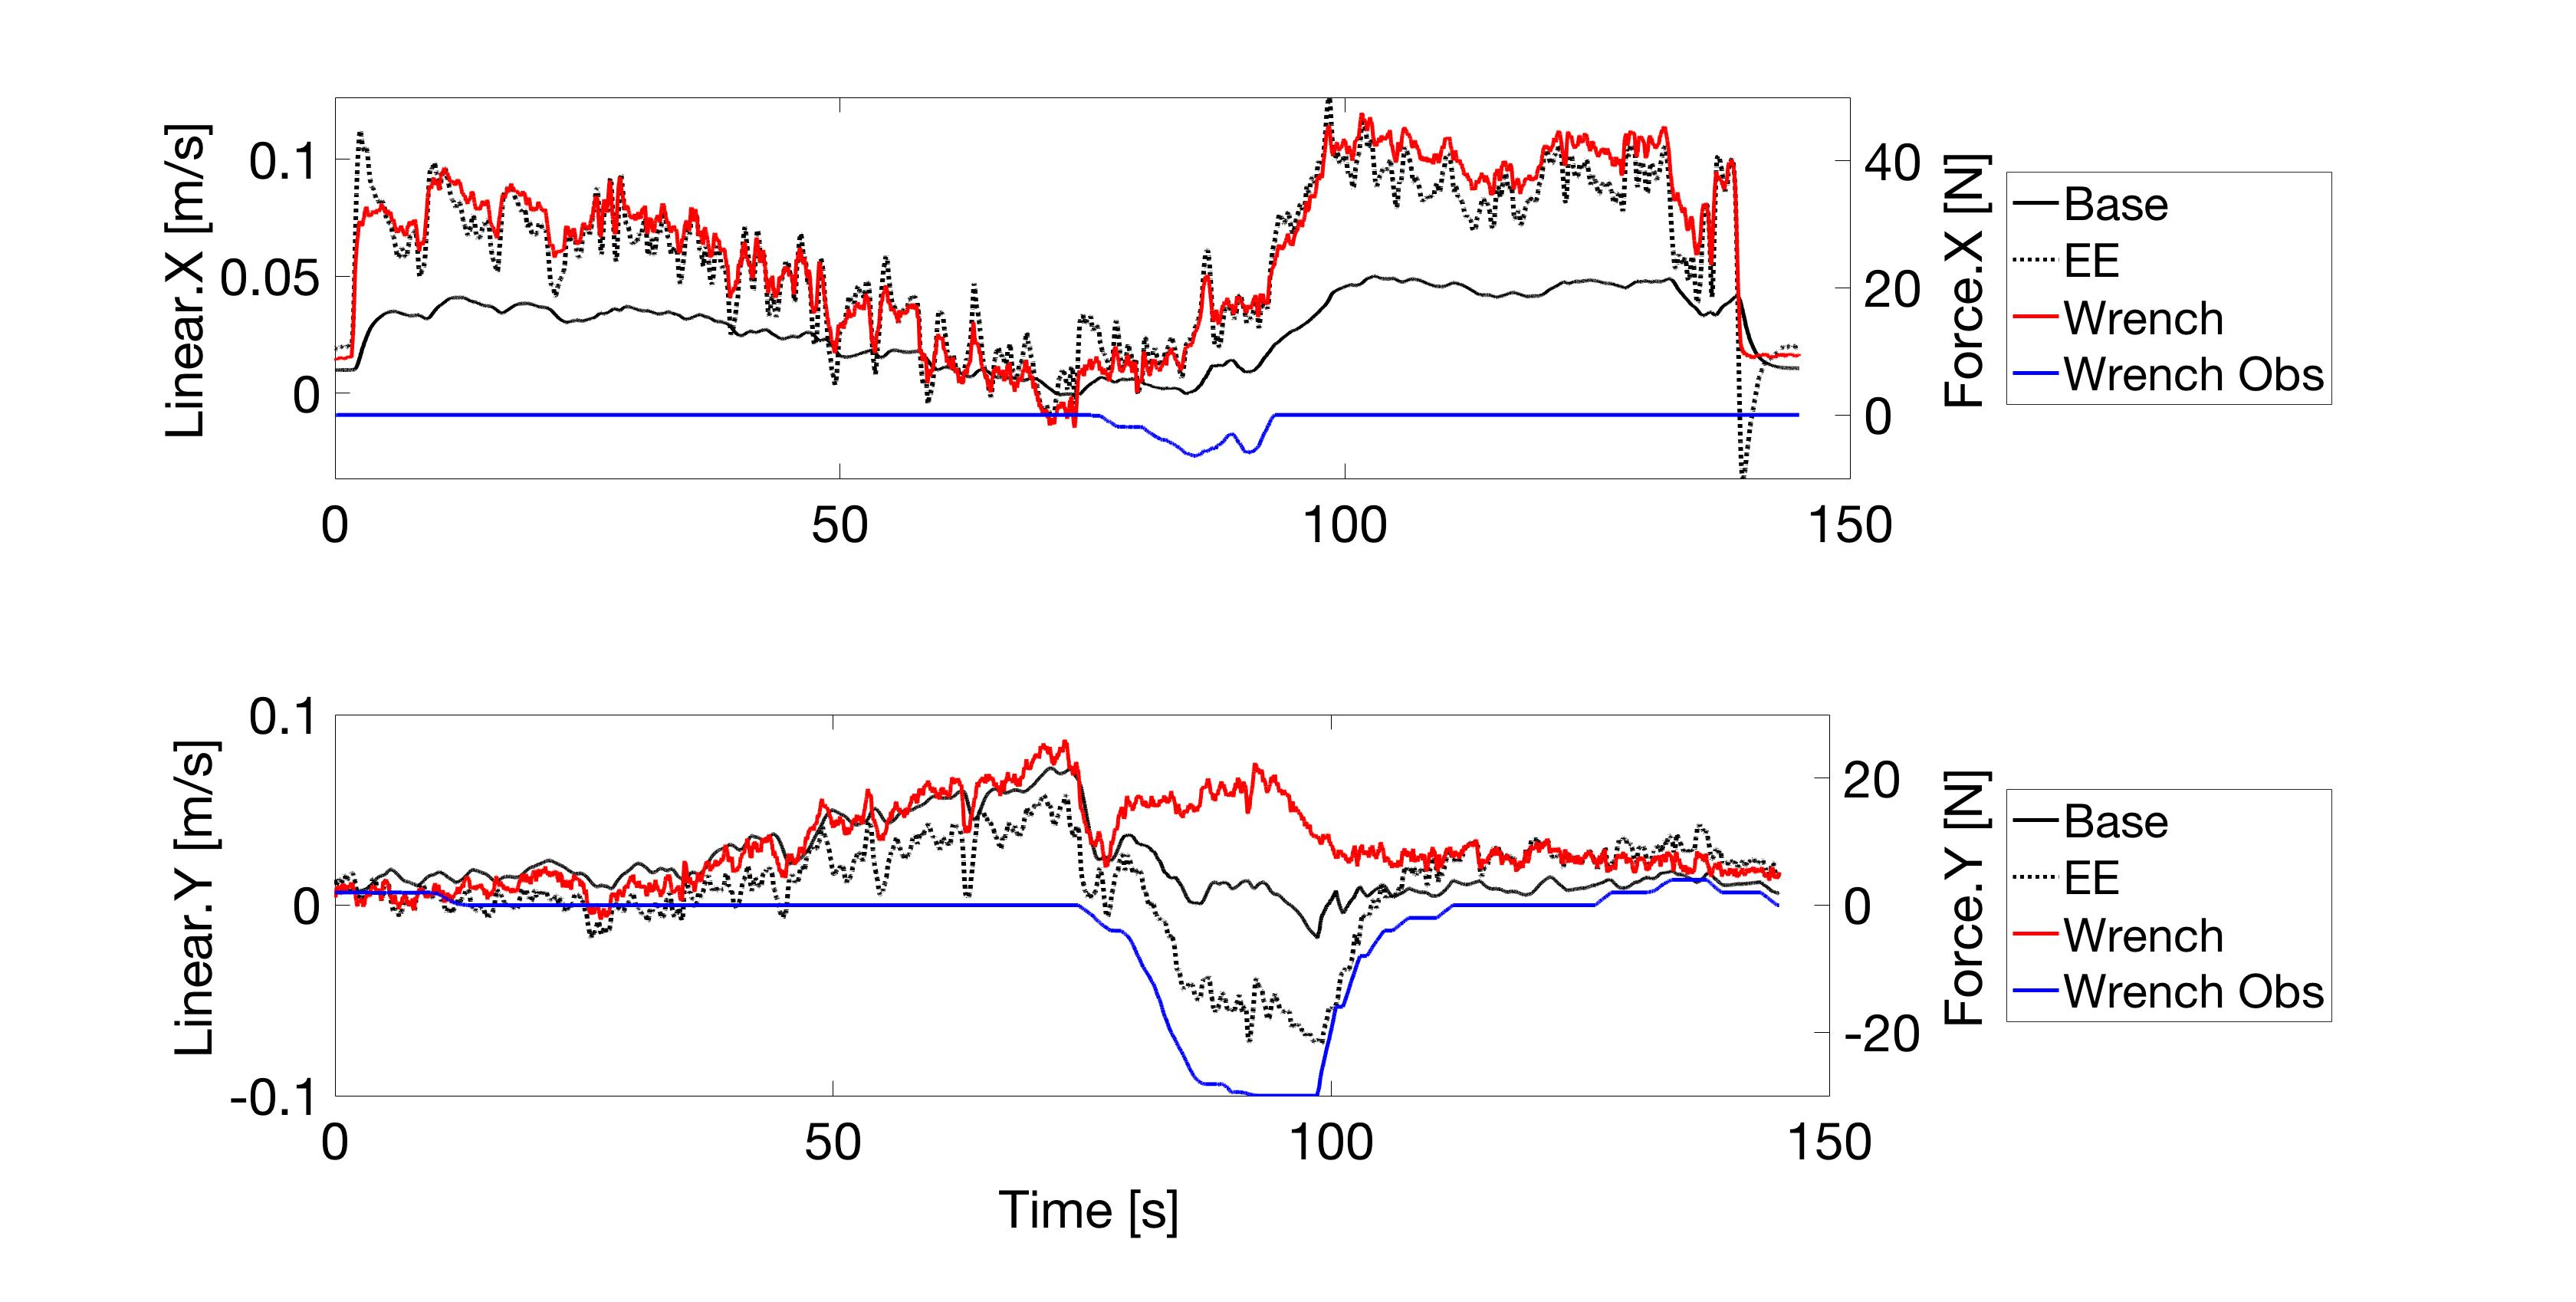
\includegraphics[width=0.75\textwidth]{images/test16.jpg}
   \caption{Velocity response to external and obstacle force input in \unit{2}{m} wide corner scenario.}
   \label{pics:test16}
\end{figure}

\subsection{Cluttered Space}
As a final experiment, we test the behaviour in a cluttered environment, as seen in Figure \ref{pics:test16_setup}. It consists of four boxes in a perpendicular arrangement with the last two boxes forming a passage of \unit[120]{cm} width.
\begin{figure}
   \centering
   \includegraphics[width=0.75\textwidth]{images/test15_setup.png}
   \caption{Execution of a test in the cluttered environment scenario.}
   \label{pics:test15_setup}
\end{figure}

\begin{figure}
   \centering
   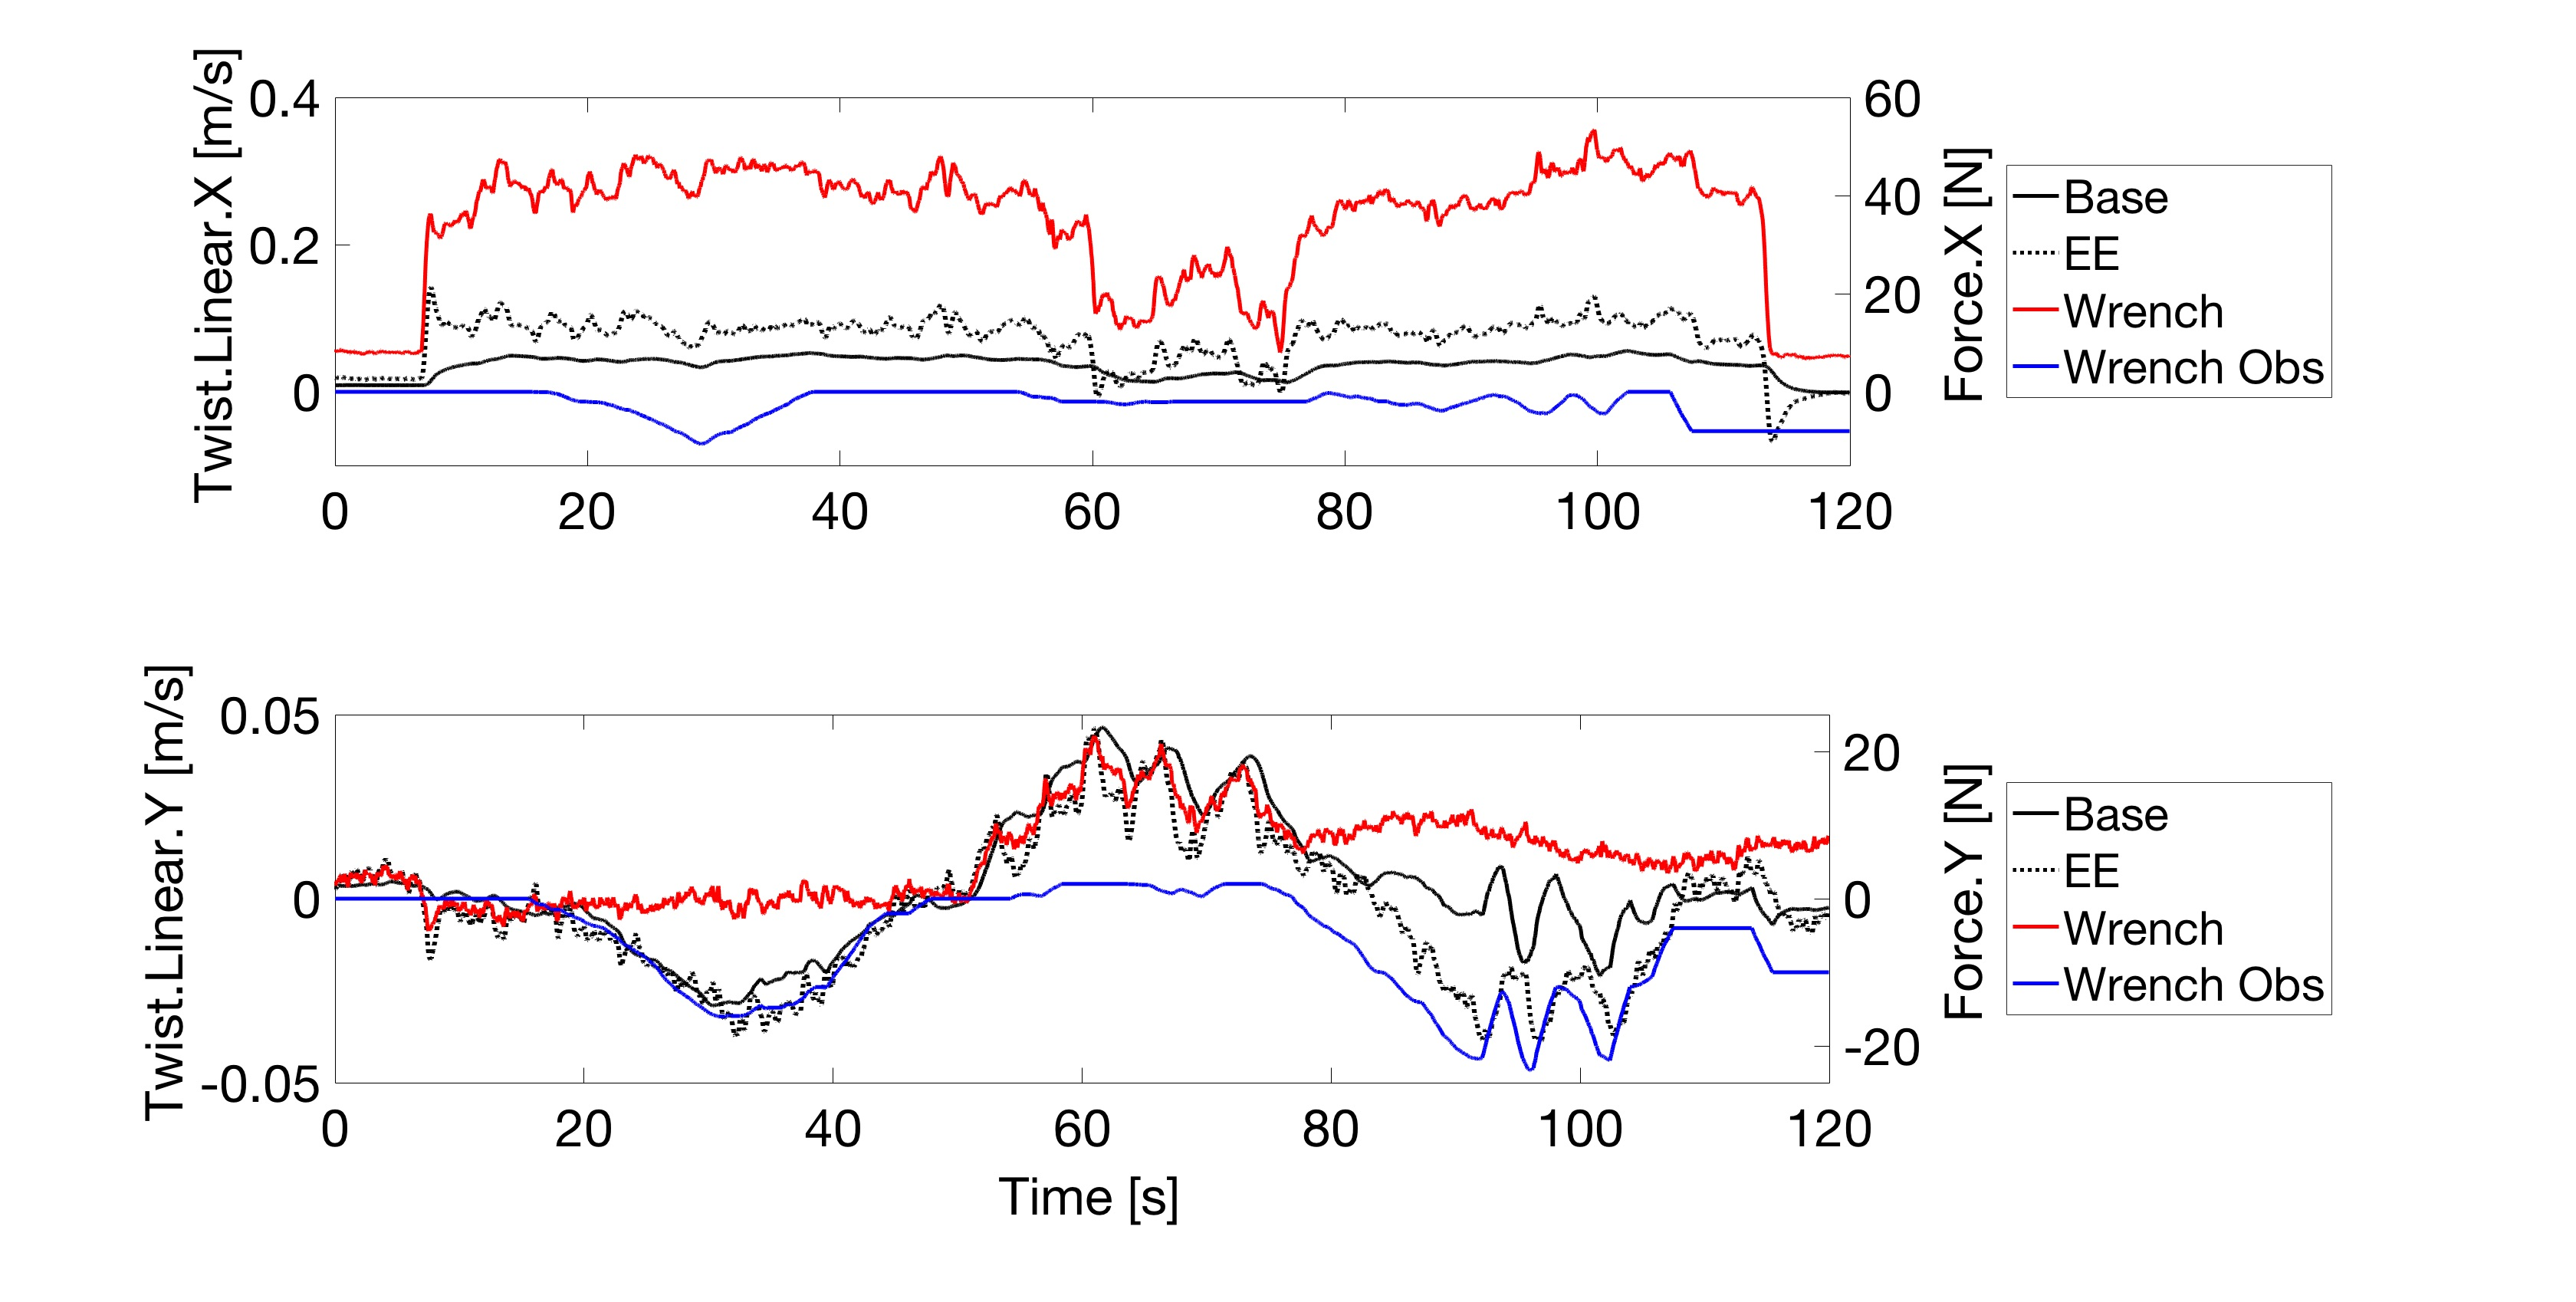
\includegraphics[width=0.75\textwidth]{images/test15_response.jpg}
   \caption{Velocity response to external and obstacle force input in the cluttered environment scenario.}
   \label{pics:test15}
\end{figure}

\chapter{Conclusion}

\chapter{Einige wichtige Hinweise zum Arbeiten mit \LaTeX\ }
\label{sec:latexumg}

Nachfolgend wird die Codierung einiger oft verwendeten Elemente
kurz beschrieben. Das Einbinden von Bildern ist in \LaTeX\ nicht
ganz unproblematisch und hängt auch stark vom verwendeten Compiler
ab. Typisches Format für Bilder in \LaTeX\ ist
EPS\footnote{Encapsulated Postscript} oder PDF\footnote{Portable Document Format}.


\section{Gliederungen}
\label{sec:gliederung}

Ein Text kann mit den Befehlen \texttt{\textbackslash
chapter\{.\}}, \texttt{\textbackslash section\{.\}},
\texttt{\textbackslash subsection\{.\}} und \texttt{\textbackslash
subsubsection\{.\}} gegliedert werden.


\section{Referenzen und Verweise}
\label{sec:refverw}

Literaturreferenzen werden mit dem Befehl \texttt{\textbackslash
citep\{.\}} und \texttt{\textbackslash
citet\{.\}} erzeugt. Beispiele: ein Buch \citep{Raibert1986LeggedRobotsThatBalance}, ein Buch und ein Journal Paper \citep{Raibert1986LeggedRobotsThatBalance,Vukobratovic2004ZeroMomentPoint}, ein Konferenz Paper mit Erwähnung des Autors: \citet{Pratt1995SEA}.

Zur Erzeugung von Fussnoten wird der Befehl \texttt{\textbackslash
footnote\{.\}} verwendet. Auch hier ein Beispiel\footnote{Bla
bla.}.

Querverweise im Text werden mit \texttt{\textbackslash label\{.\}}
verankert und mit \texttt{\textbackslash cref\{.\}} erzeugt.
Beispiel einer Referenz auf das zweite Kapitel:
\cref{sec:latexumg}.


\section{Aufzählungen}\label{sec:aufz}

Folgendes Beispiel einer Aufzählung ohne Numerierung,
\begin{itemize}
  \item Punkt 1
  \item Punkt 2
\end{itemize}
wurde erzeugt mit:
\begin{verbatim}
\begin{itemize}
  \item Punkt 1
  \item Punkt 2
\end{itemize}
\end{verbatim}

Folgendes Beispiel einer Aufzählung mit Numerierung,
\begin{enumerate}
  \item Punkt 1
  \item Punkt 2
\end{enumerate}
wurde erzeugt mit:
\begin{verbatim}
\begin{enumerate}
  \item Punkt 1
  \item Punkt 2
\end{enumerate}
\end{verbatim}

Folgendes Beispiel einer Auflistung,
\begin{description}
  \item[P1] Punkt 1
  \item[P2] Punkt 2
\end{description}
wurde erzeugt mit:
\begin{verbatim}
\begin{description}
  \item[P1] Punkt 1
  \item[P2] Punkt 2
\end{description}
\end{verbatim}


\section{Erstellen einer Tabelle}\label{sec:tabellen}

Ein Beispiel einer Tabelle:
\begin{table}[h]
\begin{center}
 \caption{Daten der Fahrzyklen ECE, EUDC, NEFZ.}\vspace{1ex}
 \label{tab:tabnefz}
 \begin{tabular}{ll|ccc}
 \hline
 Kennzahl & Einheit & ECE & EUDC & NEFZ \\ \hline \hline
 Dauer & s & 780 & 400 & 1180 \\
 Distanz & km & 4.052 & 6.955 & 11.007 \\
 Durchschnittsgeschwindigkeit & km/h & 18.7 &  62.6 & 33.6 \\
 Leerlaufanteil & \% & 36 & 10 & 27 \\
 \hline
 \end{tabular}
\end{center}
\end{table}

Die Tabelle wurde erzeugt mit:
\begin{verbatim}
\begin{table}[h]
\begin{center}
 \caption{Daten der Fahrzyklen ECE, EUDC, NEFZ.}\vspace{1ex}
 \label{tab:tabnefz}
 \begin{tabular}{ll|ccc}
 \hline
 Kennzahl & Einheit & ECE & EUDC & NEFZ \\ \hline \hline
 Dauer & s & 780 & 400 & 1180 \\
 Distanz & km & 4.052 & 6.955 & 11.007 \\
 Durchschnittsgeschwindigkeit & km/h & 18.7 &  62.6 & 33.6 \\
 Leerlaufanteil & \% & 36 & 10 & 27 \\
 \hline
 \end{tabular}
\end{center}
\end{table}
\end{verbatim}


\section{Einbinden einer Grafik}\label{sec:epsgraph}

Das Einbinden von Graphiken kann wie folgt bewerkstelligt werden:
\begin{verbatim}
\begin{figure}
   \centering
   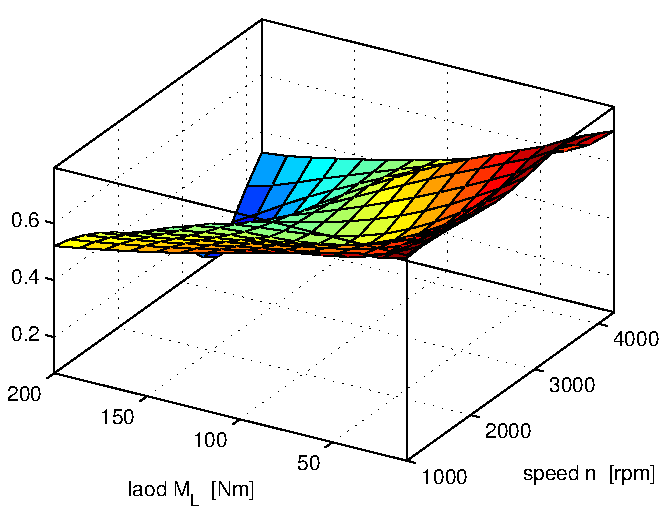
\includegraphics[width=0.75\textwidth]{images/k_surf.pdf}
   \caption{Ein Bild.}
   \label{fig:k_surf}
\end{figure}
\end{verbatim}

\begin{figure}
   \centering
   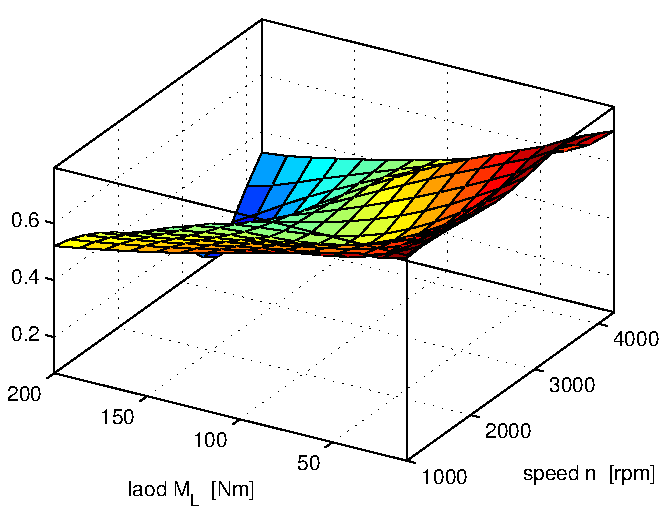
\includegraphics[width=0.75\textwidth]{images/k_surf.pdf}
   \caption{Ein Bild}
   \label{pics:k_surf}
\end{figure}

oder bei zwei Bildern nebeneinander mit:
\begin{verbatim}
\begin{figure}
  \begin{minipage}[t]{0.48\textwidth}
    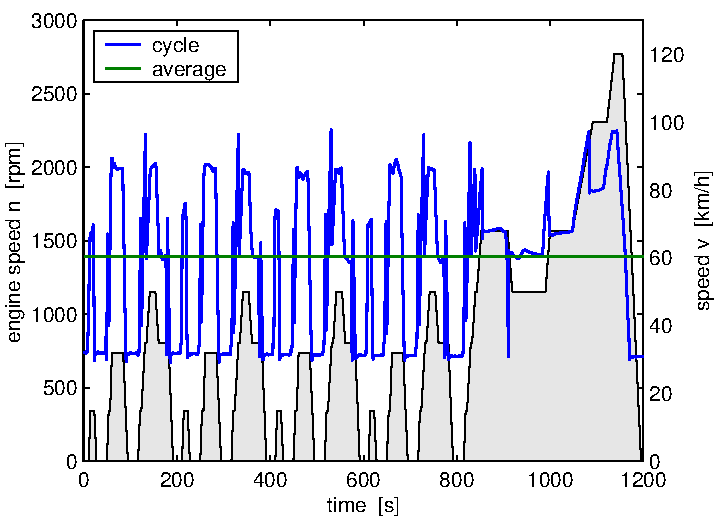
\includegraphics[width = \textwidth]{images/cycle_we.pdf}
  \end{minipage}
  \hfill
  \begin{minipage}[t]{0.48\textwidth}
    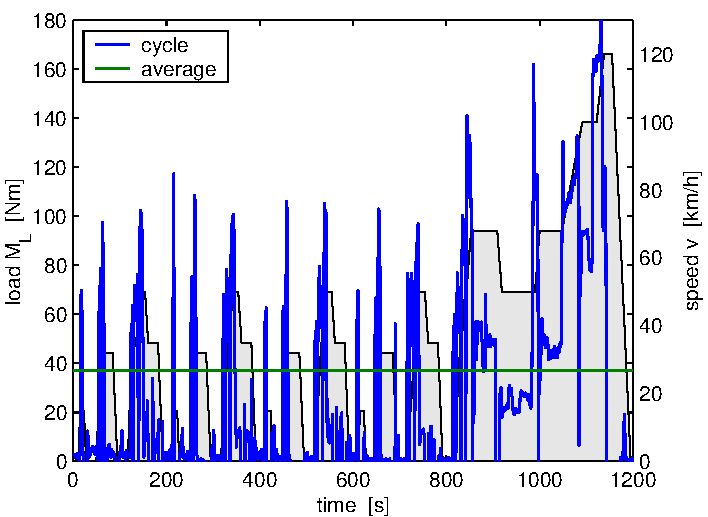
\includegraphics[width = \textwidth]{images/cycle_ml.pdf}
  \end{minipage}
  \caption{Zwei Bilder nebeneinander.}
  \label{pics:cycle}
\end{figure}
\end{verbatim}

\begin{figure}
  \begin{minipage}[t]{0.48\textwidth}
    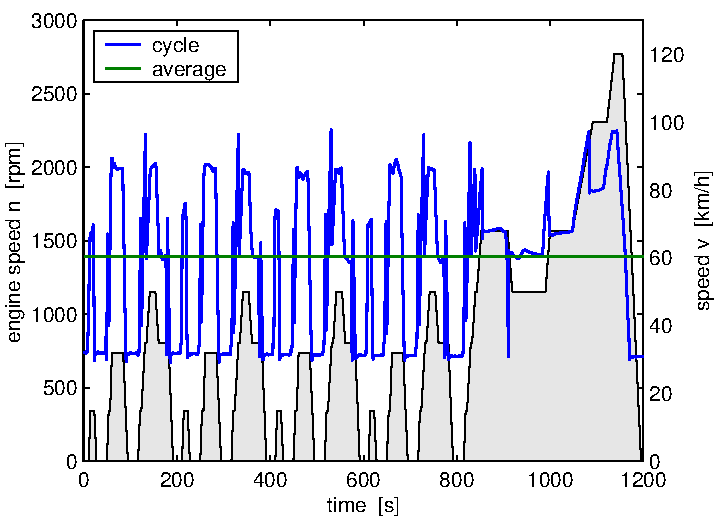
\includegraphics[width = \textwidth]{images/cycle_we.pdf}
  \end{minipage}
  \hfill
  \begin{minipage}[t]{0.48\textwidth}
    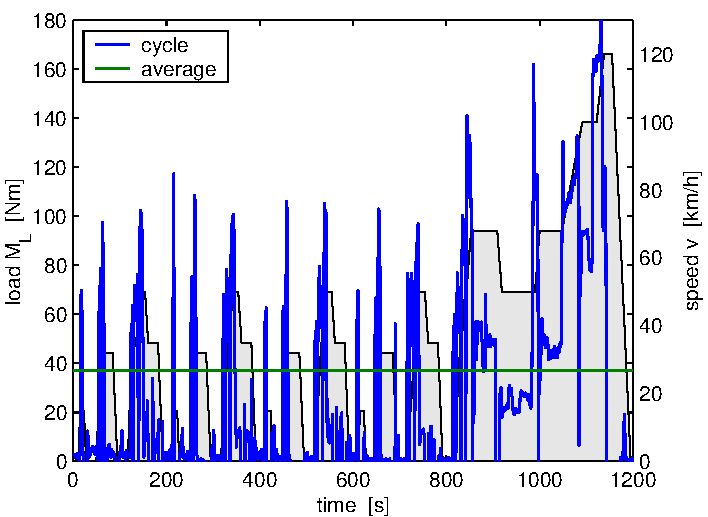
\includegraphics[width = \textwidth]{images/cycle_ml.pdf}
  \end{minipage}
  \caption{Zwei Bilder nebeneinander}
  \label{pics:cycle}
\end{figure}


\section{Mathematische Formeln}\label{sec:math}

Einfache mathematische Formeln werden mit der equation-Umgebung
erzeugt:
\begin{equation}
 p_{me0f}(T_e,\omega_e) \ = \ k_1(T_e) \cdot (k_2+k_3 S^2
 \omega_e^2) \cdot \Pi_{\mathrm{max}} \cdot \sqrt{\frac{k_4}{B}} \, .
 	\label{eq:my_equation}
\end{equation}

Der Code dazu lautet:
\begin{verbatim}
\begin{equation}
 p_{me0f}(T_e,\omega_e) \ = \ k_1(T_e) \cdot (k_2+k_3 S^2
 \omega_e^2) \cdot \Pi_{max} \cdot \sqrt{\frac{k_4}{B}} \, .
\end{equation}
\end{verbatim}

Mathematische Ausdrücke im Text werden mit \$formel\$ erzeugt (z.B.:
$a^2+b^2=c^2$).

Vektoren und Matrizen werden mit den Befehlen \texttt{\textbackslash vec\{.\}} und \texttt{\textbackslash mat\{.\}} erzeugt (z.B. $\vec{v}$, $\mat{M}$).


\section{Weitere nützliche Befehle}\label{sec:div}

Hervorhebungen im Text sehen so aus: \emph{hervorgehoben}. Erzeugt
werden sie mit dem \texttt{\textbackslash epmh\{.\}} Befehl.

Einheiten werden mit den Befehlen \texttt{\textbackslash unit[1]\{m\}} (z.B.~\unit[1]{m}) und \texttt{\textbackslash unitfrac[1]\{m\}\{s\}} (z.B.~\unitfrac[1]{m}{s}) gesetzt.
